%% abtex2-modelo-trabalho-academico.tex, v-1.9.2 laurocesar

%% Copyright 2012-2014 by abnTeX2 group at http://abntex2.googlecode.com/ 
%%
%% This work may be distributed and/or modified under the
%% conditions of the LaTeX Project Public License, either version 1.3
%% of this license or (at your option) any later version.
%% The latest version of this license is in
%%   http://www.latex-project.org/lppl.txt
%% and version 1.3 or later is part of all distributions of LaTeX
%% version 2005/12/01 or later.
%%
%% This work has the LPPL maintenance status `maintained'.
%% 
%% The Current Maintainer of this work is the abnTeX2 team, led
%% by Lauro César Araujo. Further information are available on 
%% http://abntex2.googlecode.com/
%%
%% This work consists of the files abntex2-modelo-trabalho-academico.tex,
%% abntex2-modelo-include-comandos and abntex2-modelo-references.bib
%%

% ------------------------------------------------------------------------
% ------------------------------------------------------------------------
% abnTeX2: Modelo de Trabalho Academico (tese de doutorado, dissertacao de
% mestrado e trabalhos monograficos em geral) em conformidade com 
% ABNT NBR 14724:2011: Informacao e documentacao - Trabalhos academicos -
% Apresentacao
% ------------------------------------------------------------------------
% ------------------------------------------------------------------------

\documentclass[
	% -- opções da classe memoir --
	12pt,				% tamanho da fonte
	openright,			% capítulos começam em pág ímpar (insere página vazia caso preciso)
	twoside,			% para impressão em verso e anverso. Oposto a oneside
	a4paper,			% tamanho do papel. 
	% -- opções da classe abntex2 --
	%chapter=TITLE,		% títulos de capítulos convertidos em letras maiúsculas
	%section=TITLE,		% títulos de seções convertidos em letras maiúsculas
	%subsection=TITLE,	% títulos de subseções convertidos em letras maiúsculas
	%subsubsection=TITLE,% títulos de subsubseções convertidos em letras maiúsculas
	% -- opções do pacote babel --
	english,			% idioma adicional para hifenização
	french,				% idioma adicional para hifenização
	spanish,			% idioma adicional para hifenização
	brazil				% o último idioma é o principal do documento
	]{abntex2}
%https://code.google.com/p/abntex2/wiki/Texmaker
% ---
% Pacotes básicos 
% ---
\usepackage{lmodern}			% Usa a fonte Latin Modern			
\usepackage[T1]{fontenc}		% Selecao de codigos de fonte.
\usepackage[utf8]{inputenc}		% Codificacao do documento (conversão automática dos acentos)
\usepackage{lastpage}			% Usado pela Ficha catalográfica
\usepackage{indentfirst}		% Indenta o primeiro parágrafo de cada seção.
\usepackage{color}				% Controle das cores
\usepackage{graphicx}			% Inclusão de gráficos
\usepackage{microtype} 			% para melhorias de justificação
\usepackage{url}
\usepackage[table,xcdraw]{xcolor}

% ---
		
% ---
% Pacotes adicionais, usados apenas no âmbito do Modelo Canônico do abnteX2
% ---
\usepackage{lipsum}				% para geração de dummy text
% ---

% ---
% Pacotes de citações
% ---
\usepackage[brazilian,hyperpageref]{backref}	 % Paginas com as citações na bibl
\usepackage[alf]{abntex2cite}	% Citações padrão ABNT

%%%%%%%%%%% syntax highlight %%%%%%%%%%%%%%%%%%%%%%%%%%%%%%%%%%%%%%%%%%%%%%%%%%%%%


\usepackage{listings}
\definecolor{maroon}{rgb}{0.5,0,0}
\definecolor{darkgreen}{rgb}{0,0.5,0}
\definecolor{deepblue}{rgb}{0,0,0.5}
\definecolor{deepred}{rgb}{0.6,0,0}
\definecolor{purple}{rgb}{0.5,0,0.5}
\definecolor{deepgreen}{rgb}{0,0.5,0}


 






%%%%%%%%%%%%%%%%%%%%%%%%%%%%%%%%%%%%%%%%%%%%%%%%%%%%%%% 


% --- 
% CONFIGURAÇÕES DE PACOTES
% --- 

% ---
% Configurações do pacote backref
% Usado sem a opção hyperpageref de backref
\renewcommand{\backrefpagesname}{Citado na(s) página(s):~}
% Texto padrão antes do número das páginas
\renewcommand{\backref}{}
% Define os textos da citação
\renewcommand*{\backrefalt}[4]{
	\ifcase #1 %
		Nenhuma citação no texto.%
	\or
		Citado na página #2.%
	\else
		Citado #1 vezes nas páginas #2.%
	\fi}%
% ---

% ---
% Informações de dados para CAPA e FOLHA DE ROSTO
% ---
\titulo{Luteria Composicional de algoritmos pós-tonais }
\autor{Guilherme Rafael Soares}
%\local{Brasil}
\data{10 de julho de 2014, v0.6-Qualificação}
\orientador{Prof. Dr. Daniel Quaranta}
%\coorientador{Equipe \abnTeX}
\instituicao{%
  UFJF - Universidade Federal de Juiz de Fora
  \par
  Instituto de Artes e Design
  \par
  Programa de Pós-Graduação em Artes, Cultura e Linguagens}
\tipotrabalho{Tese (Mestrado)}
% O preambulo deve conter o tipo do trabalho, o objetivo, 
% o nome da instituição e a área de concentração 
\preambulo{Prévia da dissertação para a banca de qualificação para o Mestrado em Arte, Cultura e Linguagens do IAD-UFJF.}
% ---


% ---
% Configurações de aparência do PDF final

% alterando o aspecto da cor azul
\definecolor{blue}{RGB}{41,5,195}

% informações do PDF
\makeatletter
\hypersetup{
     	%pagebackref=true,
		pdftitle={\@title}, 
		pdfauthor={\@author},
    	pdfsubject={\imprimirpreambulo},
	    pdfcreator={LaTeX with abnTeX2},
		pdfkeywords={abnt}{latex}{abntex}{abntex2}{trabalho acadêmico}, 
		colorlinks=true,       		% false: boxed links; true: colored links
    	linkcolor=blue,          	% color of internal links
    	citecolor=blue,        		% color of links to bibliography
    	filecolor=magenta,      		% color of file links
		urlcolor=blue,
		bookmarksdepth=4
}
\makeatother
% --- 

% --- 
% Espaçamentos entre linhas e parágrafos 
% --- 

% O tamanho do parágrafo é dado por:
\setlength{\parindent}{1.3cm}

% Controle do espaçamento entre um parágrafo e outro:
\setlength{\parskip}{0.2cm}  % tente também \onelineskip

% ---
% compila o indice
% ---
\makeindex
% ---

% ----
% Início do documento
% ----
\begin{document}

% Retira espaço extra obsoleto entre as frases.
\frenchspacing 

% ----------------------------------------------------------
% ELEMENTOS PRÉ-TEXTUAIS
% ----------------------------------------------------------
% \pretextual

% ---
% Capa
% ---
\imprimircapa
% ---

% ---
% Folha de rosto
% (o * indica que haverá a ficha bibliográfica)
% ---
\imprimirfolhaderosto*
% ---

% ---
% Inserir a ficha bibliografica
% ---

% Isto é um exemplo de Ficha Catalográfica, ou ``Dados internacionais de
% catalogação-na-publicação''. Você pode utilizar este modelo como referência. 
% Porém, provavelmente a biblioteca da sua universidade lhe fornecerá um PDF
% com a ficha catalográfica definitiva após a defesa do trabalho. Quando estiver
% com o documento, salve-o como PDF no diretório do seu projeto e substitua todo
% o conteúdo de implementação deste arquivo pelo comando abaixo:
%
% \begin{fichacatalografica}
%     \includepdf{fig_ficha_catalografica.pdf}
% \end{fichacatalografica}
\begin{fichacatalografica}
	\vspace*{\fill}					% Posição vertical
	\hrule							% Linha horizontal
	\begin{center}					% Minipage Centralizado
	\begin{minipage}[c]{12.5cm}		% Largura
	
	\imprimirautor
	
	\hspace{0.5cm} \imprimirtitulo  / \imprimirautor. --
	\imprimirlocal, \imprimirdata-
	
	\hspace{0.5cm} \pageref{LastPage} p. : il. (algumas color.) ; 30 cm.\\
	
	\hspace{0.5cm} \imprimirorientadorRotulo~\imprimirorientador\\
	
	\hspace{0.5cm}
	\parbox[t]{\textwidth}{\imprimirtipotrabalho~--~\imprimirinstituicao,
	\imprimirdata.}\\
	
	\hspace{0.5cm}
		1. Palavra-chave1.
		2. Palavra-chave2.
		I. Orientador: Prof. Dr. Daniel Quaranta
		II. UFJF - Universidade Federal de Juiz de Fora.
		III. Instituto de Artes e Design
		IV. \imprimirtitulo \\ 			
	
	\hspace{8.75cm} CDU 02:141:005.7\\
	
	\end{minipage}
	\end{center}
	\hrule
\end{fichacatalografica}
% ---

% ---
% Inserir errata
% ---
%\begin{errata}
%Elemento opcional da \citeonline[4.2.1.2]{NBR14724:2011}. Exemplo:
%
%\vspace{\onelineskip}
%
%FERRIGNO, C. R. A. \textbf{Tratamento de neoplasias ósseas apendiculares com
%reimplantação de enxerto ósseo autólogo autoclavado associado ao plasma
%rico em plaquetas}: estudo crítico na cirurgia de preservação de membro em
%cães. 2011. 128 f. Tese (Livre-Docência) - Faculdade de Medicina Veterinária e
%Zootecnia, Universidade de São Paulo, São Paulo, 2011.
%
%\begin{table}[htb]
%\center
%\footnotesize
%\begin{tabular}{|p{1.4cm}|p{1cm}|p{3cm}|p{3cm}|}
%  \hline
%   \textbf{Folha} & \textbf{Linha}  & \textbf{Onde se lê}  & \textbf{Leia-se}  \\
%    \hline
%    1 & 10 & auto-conclavo & autoconclavo\\
%   \hline
%\end{tabular}
%\end{table}

%\end{errata}
% ---

% ---
% Inserir folha de aprovação
% ---

% Isto é um exemplo de Folha de aprovação, elemento obrigatório da NBR
% 14724/2011 (seção 4.2.1.3). Você pode utilizar este modelo até a aprovação
% do trabalho. Após isso, substitua todo o conteúdo deste arquivo por uma
% imagem da página assinada pela banca com o comando abaixo:
%
% \includepdf{folhadeaprovacao_final.pdf}
%
\begin{folhadeaprovacao}

  \begin{center}
    {\ABNTEXchapterfont\large\imprimirautor}

    \vspace*{\fill}\vspace*{\fill}
    \begin{center}
      \ABNTEXchapterfont\bfseries\Large\imprimirtitulo
    \end{center}
    \vspace*{\fill}
    
    \hspace{.45\textwidth}
    \begin{minipage}{.5\textwidth}
        \imprimirpreambulo
    \end{minipage}%
    \vspace*{\fill}
   \end{center}
        
   Trabalho aprovado \imprimirlocal, 13 de fevereiro de 2015:

   \assinatura{\textbf{\imprimirorientador} \\ Orientador} 
   \assinatura{\textbf{Professor} \\ Convidado 1}
   \assinatura{\textbf{Professor} \\ Convidado 2}
   %\assinatura{\textbf{Professor} \\ Convidado 3}
   %\assinatura{\textbf{Professor} \\ Convidado 4}
      
   \begin{center}
    \vspace*{0.5cm}
    {\large\imprimirlocal}
    \par
    {\large\imprimirdata}
    \vspace*{1cm}
  \end{center}
  
\end{folhadeaprovacao}
% ---

% ---
% Dedicatória
% ---
%\begin{dedicatoria}
%   \vspace*{\fill}
%   \centering
%   \noindent
%   \textit{ Este trabalho é dedicado às crianças adultas que,\\
%   quando pequenas, sonharam em se tornar cientistas.} \vspace*{\fill}
%\end{dedicatoria}
% ---

% ---
% Agradecimentos
% ---
%\begin{agradecimentos}

%A você...\footnote{...principalmente pela atenção até nas notas de rodapé.}



%\end{agradecimentos}
% ---

% ---
% Epígrafe cortazar
% ---
%\begin{epigrafe}
%    \vspace*{\fill}
%	\begin{flushright}
%		\textit{``Quantas vezes me pergunto se isto não é mais do que escrita, numa época em que corremos para o %engano entre equações infalíveis e máquinas de conformismos? Mas perguntar se saberemos encontrar o outro lado do %hábito ou se mais vale se deixar levar pela sua alegre cibernética, não será mais uma vez literatura? Revolta, %conformismo, angústia, alimentos terrestres, todas as dicotomias: o Yin e o Yang, a contemplação (...) e, %finalmente; um encolher de ombros, a paz, o parafuso foi a paz, ninguém podia passar pela rua sem olhar de soslaio %para o parafuso e sentir que ele era a paz. \cite{cortazar1963} }
%	\end{flushright}
%\end{epigrafe}



% ---

% ---
% RESUMOS
% ---

% resumo em português
\setlength{\absparsep}{18pt} % ajusta o espaçamento dos parágrafos do resumo
\begin{resumo}


Esta pesquisa visa problematizar e sistematizar um catálogo de experimentos constituído de pequenas peças musicais e seus algoritmos geradores, objetivando a construção de uma biblioteca de objetos para composição assistida por computador que gere partituras baseadas em pequenas regras extraídas de análises.

Formalizamos tais aspectos através de um estudo comparado de dois paradigmas de análise musical aplicáveis a estas peças: "A Teoria Gerativa da Música Tonal"\cite{lerdahl1983generative} com algumas de suas continuidades propostas \cite{lerdahl2009genesis,temperley2001cognition} e a teoria dos conjuntos e classes de alturas cromáticas.\cite{forte1973structure,straus2004}

Os procedimentos utilizados são derivados de aspectos intervalares singulares encontrados em algumas peças da suíte Mikrokosmos do compositor Béla Bartók. Este repertório foi escolhido devido a seu reconhecido contexto como composições pianísticas e pedagógicas situadas nas fronteiras da pós-tonalidade. 

Apontamos as limitações encontradas na aplicação dos paradigmas analíticos adotados aqui no contexto da suíte de peças escolhidas e suas derivações composicionais.

Detalhamos questões computacionais para esta implementação e deixamos um legado de código aberto para continuidades possíveis deste trabalho.


 \textbf{Palavras-chaves}: Música algorítmica. Pós-tonalismo. Teoria dos conjuntos. Pitch class theory. Luteria. Composição assistida por computador. Cibernética. Software livre. Cognição musical.
\end{resumo}

%%%%%%%%%% traduçoes resumo
\begin{comment}
% resumo em inglês
\begin{resumo}[Abstract]
 \begin{otherlanguage*}{english}
   This is the english abstract.

   \vspace{\onelineskip}
 
   \noindent 
   \textbf{Key-words}: latex. abntex. text editoration.
 \end{otherlanguage*}
\end{resumo}

% resumo em francês 
\begin{resumo}[Résumé]
 \begin{otherlanguage*}{french}
    Il s'agit d'un résumé en français.
 
   \textbf{Mots-clés}: latex. abntex. publication de textes.
 \end{otherlanguage*}
\end{resumo}

% resumo em espanhol
\begin{resumo}[Resumen]
 \begin{otherlanguage*}{spanish}
   Este es el resumen en español.
  
   \textbf{Palabras clave}: latex. abntex. publicación de textos.
 \end{otherlanguage*}
\end{resumo}
% ---
\end{comment}


% ---
% inserir lista de ilustrações
% ---
\pdfbookmark[0]{\listfigurename}{lof}
\listoffigures*
\cleardoublepage
% ---

% ---
% inserir lista de tabelas
% ---
%\pdfbookmark[0]{\listtablename}{lot}
%\listoftables*
%\cleardoublepage
% ---

% ---
% inserir lista de abreviaturas e siglas
% ---
\begin{siglas}
  \item[GTTM] Generative Theory of Tonal Music\footnote{ "Teoria Gerativa da Música Tonal"      \cite{lerdahl1983generative} }
  \item[TPS] Tonal Pitch Space\footnote{ "Espaço das Alturas Tonais"\cite{lerdahl1988tps} }
  \item[CBMS] Cognition of Basic Musical Structures\footnote{ "Cognição das Estruturas Musicais Básicas"\cite{temperley2001cognition} }
\end{siglas}
% ---

% ---
% inserir lista de símbolos
% ---
%\begin{simbolos}
%  \item[$ \Gamma $] Letra grega Gama
%  \item[$ \Lambda $] Lambda
%  \item[$ \zeta $] Letra grega minúscula zeta
%  \item[$ \in $] Pertence
%\end{simbolos}
% ---

% ---
% inserir o sumario
% ---
\pdfbookmark[0]{\contentsname}{toc}
\tableofcontents*
\cleardoublepage
% ---

%
%
%
%
%
%
%
% ----------------------------------------------------------
% ELEMENTOS TEXTUAIS
% ----------------------------------------------------------
\textual

% ----------------------------------------------------------
% Introdução (exemplo de capítulo sem numeração, mas presente no Sumário)
% ----------------------------------------------------------
\chapter*[Introdução]{Introdução}
\addcontentsline{toc}{chapter}{Introdução}
% ----------------------------------------------------------

%\citeonline{adorno1974filosofia}


Desde o momento em que o computador emancipa-se do estúdio experimental e seus aparelhos caros e institucionais e possibilita o processamento de dados em tempo real em gadgets que cabem no nosso bolso (e cada vez mais até dentro dos nossos corpos) fala-se constantemente na possibilidade de interação com a transformação de dados audiovisuais através de uma computabilidade da escritura composicional ou do gestual performático. 

Em seu livro sobre mediação tecnológica contemporânea na composição Fernando \citeonline{iazzetta2009musica} fala sobre um tipo de \textit{\textbf{"luteria composicional"}} que surge do experimento de estúdio migrando para os computadores pessoais, onde a criação dos instrumentos (que na verdade são códigos, procedimentos computacionais, "patches") agora já fariam parte do processo composicional:


\begin{citacao}
“Mesmo porque, muitas vezes, o trabalho de composição se confunde com o trabalho de criação dos instrumentos que serão usados na composição. O conhecimento do funcionamento interno destes instrumentos e a possibilidade de correção e aperfeiçoamento constante assim como o acoplamento de novas interfaces ao sistema, confere ao compositor um domínio maior da execução da sua obra”  \cite[p. 209]{iazzetta2009musica}.
\end{citacao}

Por outro lado, o fechamento deste processo em \textit{"microteorias composicionais derivadas da circulação dos manuais de softwares musicais"}\cite[p. 152]{iazzetta2009musica} não parecem serem suficientes para dar conta de uma série de procedimentos composicionais que existiam muito antes de serem pensados a priori já por dentro destes sistemas.

\begin{citacao}
"Qualquer estrutura, gramática ou modelo pode, em princípio, ser transposto para o âmbito sonoro com a intenção de produzir música. Uma vez que nos sistemas computacionais todo e qualquer elemento é transcrito na forma de símbolos abstratos do mesmo tipo (em última instância, bits representados por 0 e 1), esse tipo de procedimento se torna tentador, mas também vulnerável.(...)Certamente estas transposições de um campo a outro não destroem a coerência interna dos fenômenos transpostos, mas de forma alguma asseguram a  geração de uma coerência musical, pelo menos não no nível perceptivo.
(...)
\textbf{O discurso enfatizando o caráter inovador que acompanha cada novo invento geralmente esconde o quanto nossos avanços representam uma consolidação  de conhecimentos existentes, mais do que saltos progressivos}”. \cite[p. 151-153, grifo nosso.]{iazzetta2009musica}
\end{citacao}

Esta pesquisa propõe um recorte específico de alguns procedimentos composicionais emergentes na primeira metade do século XX, que estão no limite entre o politonalismo e o atonalismo, sob a luz de teorias que influenciaram a criação de algoritmos de análise musical assistida por computador nas décadas mais recentes. 

Os problemas computacionais considerados no percurso compõem uma suíte de objetos e funções organizados em bibliotecas para as linguagens de programação musical OpenMusic e Puredata, facilita-se assim um estudo comparado das implementações dos procedimentos algorítmicos em diferentes sintaxes. As composições geradas pelo processo fomentam nova reflexão sobre o automatismo e interação dentro de seus procedimentos.

Complementamos o trabalho com a documentação de scripts Python auxiliares para formatação e segmentação de partituras (em formatos midi, musicxml ou lilypond, dependendo do caso).

O percurso deste trabalho se dá em duas etapas: \autoref{analises}:\textbf{Paradigmas para uma Análise Musical Pós-Tonal} e \autoref{computacional}:\textbf{Implementação Computacional}.

Na \autoref{analises} buscamos organizar bases para análises computacionais do processo criativo traçando uma epistemologia das gramáticas musicais a partir da influência que a linguística teve na musicologia. Atentamos para as teorias derivadas da pesquisa de \citeonline{chomsky1957syntactic} e sua aplicação no processamento de linguagens naturais. Buscamos aspectos que direcionaram pesquisas musicológicas para a possibilidade de aplicar regras analíticas em sistemas computáveis.

A partir dessas perspectivas, encontramos duas abordagens analíticas que nos chamaram atenção por serem relativamente contemporâneas entre si e que partem de diferentes princípios. 

A primeira abordagem é a da \textit{"Teoria Gerativa da Música Tonal"}\cite{lerdahl1983generative} e alguns desdobramentos mais recentes como a \textit{"Cognição das Estruturas Musicais Básicas"}\cite{temperley2001cognition} para buscar algoritmos que definam critérios quantitativos para análises tomem em consideração a normatização operada pela música tonal ocidental na percepção do seu ouvinte médio. Estas teorias flertam com argumentos da psicologia cognitivista da música\cite{krumhansl1990cognitive} para justificar seus pressupostos.

A segunda é a corrente musicológica que trabalha sobre um mapeamento dos agrupamentos de classes de alturas, organizando taxonomias \cite{forte1973structure}, descrevendo operações de transformação\cite{straus2004} e buscando critérios mais autorais para apontar singularidades em composições\cite{lester1989analytic,straus2004} que não necessariamente operam sobre os pressupostos de uma expectativa de tonalidade explícita.

Na \autoref{computacional} trabalhamos uma reflexão sobre procedimentos, formatos de arquivos e bibliotecas de linguagem de programação para uma \textit{"Composição Assistida por Computador"}(CAC) usadas durante esta pesquisa. Bases para implementação dos estudos da \autoref{analises}.
\linebreak
\linebreak
\linebreak
E finalmente na conclusão\footnote{ ver \autoref{conclusao}} deste trabalho utilizaremos algumas ideias e particularidades retiradas dos procedimentos analíticos detalhados na \autoref{analises} para construir composições musicais que aplicam estruturas destacadas das análises de Mikrokosmos de Béla Bartók, usando as implementações computacionais que nos pareceram mais estáveis e bem documentadas.























% ----------------------------------------------------------
% PARTE
% ----------------------------------------------------------
\part{Paradigmas para uma Análise Musical Pós-Tonal}
\label{analises}
% ----------------------------------------------------------




% ---
% Capitulo de revisão de literatura
% ---
\chapter{Teorias Cognitivistas para uma Segmentação Tonal}

\section{Formalização linguística de gramáticas musicais }

Em seu ensaio "A comparação das análises sob o ponto de vista semiológico", J.J. \citeonline{nattiezcomparaccao} faz um balanço das diferentes abordagens analíticas na musicologia 

\begin{citacao}
As diversas práticas da análise musical no século XX podem, na minha opinião, estar, de início, repartidas em duas grandes categorias, (...): 

1. Aquelas que admitem – e mesmo sublinham – as conotações emotivas, afetivas, imagéticas da obra musical. Designarei as mesmas com o termo genérico e moderno de análises de orientação semântica. (...)\linebreak
2. Aquelas que se apoiam sobre as estruturas imanentes da obra e que se repartem em dois grandes grupos: a. \textbf{as análises taxionômicas que cortam em unidades a substância musical, privilegiando este ou aquele parâmetro. }(...) b. \textbf{As análises que, na falta de melhor termo, chamarei “lineares” e que, (...), 
descrevem o prolongamento e as implicações das alturas, tanto no nível melódico (...), quanto no harmônico (...)}
\cite[grifos nossos]{nattiezcomparaccao}
\end{citacao}


% ---
A segunda categoria apontada por Nattiez, \textbf{uma análise focada nas estruturas sintáticas}, é o foco desta parte da pesquisa.

Tentando compreender a influência desta oposição entre sintaxe e semântica nas análises musicais, buscamos as origens deste estudo comparado de linguística e gramáticas musicais.

O modelo de racionalização da linguística iniciado por Noam Chomsky com a obra \textit{"Syntactic Structures"} \cite{chomsky1957syntactic} e formalizado na sua \textit{"Teoria da Sintaxe"}\cite{chomsky1965aspects}  até hoje é uma das bases para o estudo algorítmico e algébrico de processamento linguagens naturais.  

Sua influência na teoria musical pode ser encontrada em muitas tentativas de aproximar linguística e musicologia nas década de 70 e 80.\cite{roads1978composing}

Inspirou as formalizações rígidas de modelos da musicologia da cognição inspirados na linguística, como na \textit{“Teoria Gerativa da Música Tonal”} \cite{lerdahl1983generative} - um trabalho interdisciplinar do linguista Ray Jackendoff com o musicólogo Fred Lerdahl que detalharemos mais adiante.

Uma das primeiras comparações entre as teorias sintáticas de Chomsky e análises musicais é a de Leonard Bernstein na série de palestras \textit{“Unanswered Question”} \cite{bernstein1976unanswered}. Sua especulação empírica foi bastante alegórica e demonstrada inventivamente ao piano em seu registro em vídeo. Bernstein fez comparações das estruturas de ordenamento das frases escritas e faladas com montagens de sessões motívicas de peças clássicas e chega a fazer algumas metáforas entre classes gramaticais e funções de acordes. Este tipo de metáfora parece ser de fato uma das motivações iniciais da pesquisa neste campo, porém muita coisa foi problematizada de maneira mais rigorosa, buscando métodos quantitativos, e nos anos seguintes contribuiu para as bases de organização de uma disciplina hoje conhecida por cognição musical.

Pelo bem ou pelo mal, a abordagem de Bernstein parecia estar muito mais para o universo das analogias poéticas livres do que a busca por uma formalização strictu sensu.
 

\section{Gramáticas Musicais Computáveis}

Uma interessante e histórica análise strictu sensu sobre a influência da linguística computacional na musicologia está no ensaio \textit{"Grammars as representations for music"}  de Curtis \citeonline{roads1979grammars}. O ensaio é um panorama sobre o estado da arte da influência da linguística sobre musicologia na época, um estudo comparado dos trabalhos de \citeonline{smoliar1976music,lindblom1970towards,laske1977music, winograd1968linguistics, moorer1972music, nattiez1977fondements,ruwet1975theorie, lerdahl1983generative} e o próprio trabalho anterior de \citeonline{roads1978composing}.


O interessante deste panorama é que coloca lado a lado perspectivas mais empíricas como de \citeonline{nattiez1977fondements} e \citeonline{ruwet1975theorie} e outras que buscavam efetivamente uma inspiração para um rigor computacional de sintaxes musicais. Vale lembrar que Nattiez também tem um estudo comparado da influência da linguística na musicologia, com um ponto de vista menos pragmático e mais historicista, muito mais abrangente, e que traz um ponto de vista bem mais recente \cite{nattiez2004modelos}.


Segundo Roads, \citeonline{moorer1972music} e \citeonline{winograd1968linguistics} chegam a realizar alguns experimentos computacionais. \citeonline{smoliar1976music} toca num ponto tecnologicamente complexo para a época: a segmentação de arquivos sonoros diretamente a partir de gravações. 

\citeonline{laske1977music} propõe analogias com a fonologia (relação entre sintaxe e sons da palavra falada) com uma recente “sonologia” (relação de uma sintaxe musical e os sons musicais). 

Já a dupla \citeonline{lerdahl1983generative}  investe numa normatização bastante inspirada nas segmentações propostas por Chomsky e procura problematizar aspectos de uma cognição musical tonal - que teria bases culturais sólidas na tradição ocidental. Seguiremos este percurso logo a seguir.





\section{Gramática Gerativa da Música Tonal (GTTM)}
\label{GTTM}

Jean Jaques Nattiez, em seu ensaio sobre música e linguística \cite{nattiez2004modelos} relativiza o êxito do texto de Lerdahl e Jackendoff, porém reconhece uma importância  que despertou nossa curiosidade por uma pequena revisão nas regras propostas por esta obra.

\begin{citacao}
Porque, se a obra de Lerdahl e Jackendoff não conheceu um amplo reconhecimento sob o ponto de vista da análise das obras stricto sensu, em compensação, a \textbf{psicologia cognitiva da música, que sabemos estar em plena efervescência, dela se apossou. (...) Na medida em que 51 das 56 regras propostas são dadas como universais \cite[ p.345-352]{lerdahl1983generative}, os autores lançam aos etnomusicólogos um grande e salutar desafio que ainda não foi levado em consideração.} A importância de um trabalho não se mede unicamente por seu caráter inovador e pelo valor dos modelos propostos, o que, por certo, ocorre neste caso, mas também pelo campo de investigações novas que propõe.
\cite[ grifos nossos.]{nattiez2004modelos}
\end{citacao}

A \textit{"Generative Theory of Tonal Music"}\cite{lerdahl1983generative} \footnote{Doravante tratada por GTTM.} introduz uma taxonomia para separar de um plano musical seus agrupamentos melódicos, harmônicos e rítmicos, buscando uma maneira estruturada para fazer uma segmentação hierárquica de motivos que supostamente estariam dentro de uma previsibilidade de uma escuta ocidental tonal. Ela aponta limitações e contradições entre estas regras e buscando apoiar-se em processos cognitivos rastreados pela audição, psicoacústica e cultura desta escuta.\footnote{
Lerdahl e Jackendoff colocam o termo “regra gerativa”\ ( que é derivado da linguística ) significando uma estrutura pela qual a escuta já experimentada naquela cultura musical guia-se para segmentar e fruir sua sixtaxe. \cite[ p.6]{lerdahl1983generative}
}.  



%%%%%%%%%%%%%%%%%% gttm esquema
\begin{figure}[!h]
	\caption{\label{fig_grafico}Fluxograma de \citeonline{lerdahl2009genesis} para a GTTM}
	\begin{center}
	    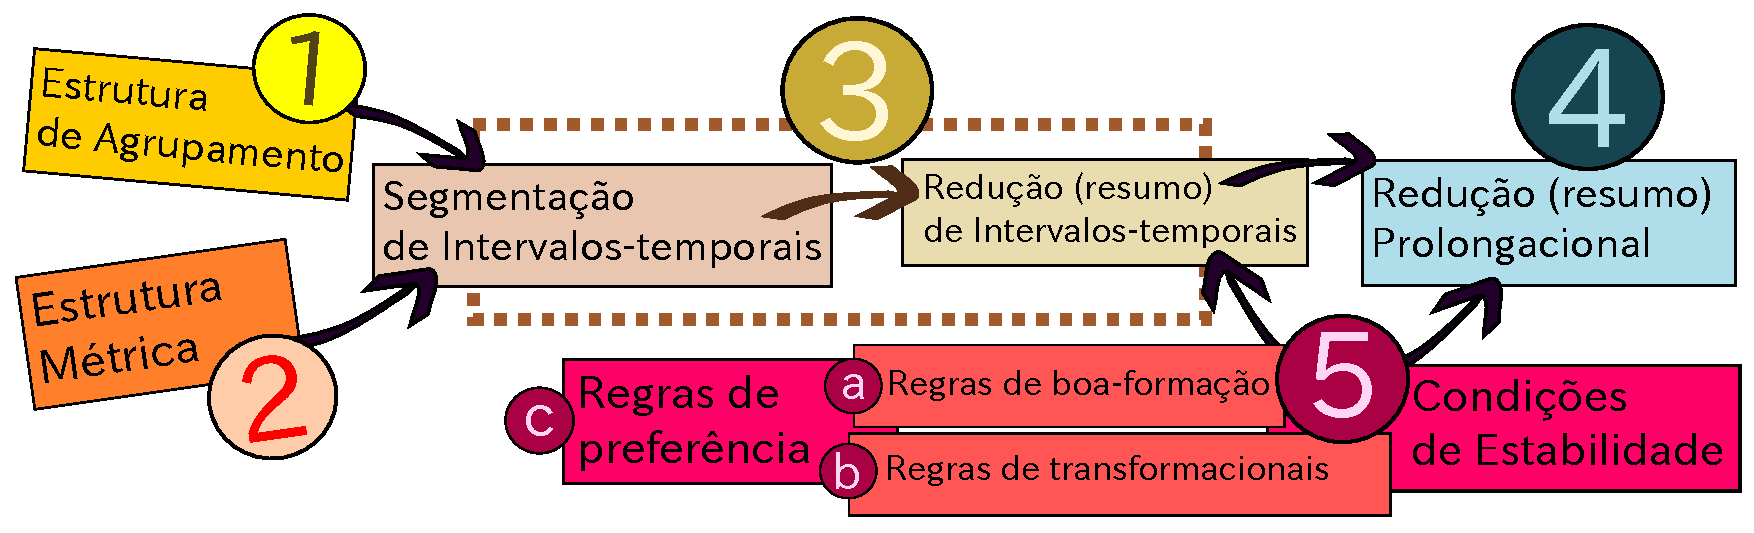
\includegraphics[scale=0.5]{gttm/GTTM_rules.pdf}
	\end{center}
	\legend{Fonte: \citeonline[p. 2 , tradução do autor]{lerdahl2009genesis}}
\end{figure}

\pagebreak
Em revisões que sucedem a GTTM, Fred Lerdahl desenha o esquema básico do seu funcionamento dividindo-a em quatro estruturas:

\begin{citacao}
A teoria [GTTM] clama que, se um sinal permite, o ouvinte inconscientemente infere quatro tipos de estruturas hierárquicas de uma superfície musical:\linebreak 
\textbf{1. estrutura de agrupamento}, ou a segmentação do fluxo musical em unidades como motivos, frases e sessões; 
\textbf{2. estrutura métrica}, ou padrão de batidas recorrentes periodicamente forte e fracas associadas com a superfície; 
\textbf{3. redução de intervalo temporal}, ou a importância estrutural relativa dos eventos como são ouvidos dentro do contexto estabelecido pelas unidades rítmicas; e
\textbf{4. redução prolongacional}, ou os padrões percebidos pela tensão e relaxamento ao longo dos eventos em vários níveis da estrutura \cite{lerdahl1992cognitive}
\footnote{
"The theory claims that, if the signal permits, the listener unconsciously infers four types of hierarchical structure from a musical surface: grouping structure, or the segmentation of the musical flow into units such as motives, phrases, and sections; metrical structure, or the pattern of periodically recurring strong and weak beats associated with the surface; time-span reduction, or the relative structural importance of events as heard within contextually established rhythmic units; and prolongational reduction, or the perceived pattern of tension and relaxation among events at various levels of structure"\cite{lerdahl1992cognitive}

}
\end{citacao}

O quinto elemento da Figura 1, as "regras de preferência", seriam compostas pelas condições de estabilidade das 4 estruturas: regras de "boa-formação"\ que são mais essenciais para a segmentação básica e as "regras de preferencia"\ hierarquizadas pelo contexto.


\subsection{Estrutura de Agrupamento}

As regras de boa formatividade dos agrupamentos \textit{("Grouping Well-Formed Rules" - GWFRs) }definem o conjunto mais geral e axiomático das regras da GTTM, definindo premissas como o fato de que a análise considera uma escuta linear e hierarquizada, com pequenos grupos interdependentes de seus prolongamentos em grandes grupos.

%%%%%%%%%%%%%%%%%% mozart
\begin{figure}[htb]
	\caption{\label{fig_grafico}Agrupamento de motivos do início da sinfonia K550 de Mozart.}
	\begin{center}
	    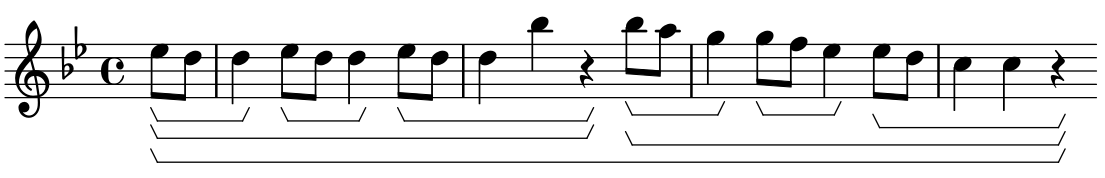
\includegraphics[scale=0.45]{gttm/lilypondGROUPmozartGTTM.png}
	\end{center}
	\legend{Fonte: \cite{lerdahl1983generative} }
\end{figure}

\begin{citacao}
\textbf{GWFR 1} “Qualquer sequencia contígua de eventos de alturas, batidas percussivas, ou similares constituem um grupo, e somente sequencias contíguas constituem um grupo” \cite[ pg.37]{lerdahl1983generative}.
\end{citacao}

Esta regra estabelece que esse tipo de escuta irá selecionar agrupamentos apenas por eventos sequenciados, não valendo por exemplo agrupar sons apenas por estarem na mesma oitava ou por serem de figuras rítmicas iguais figurando em diferentes sessões da peça, pois isto implicaria uma seleção cognitiva-auditiva de eventos num tempo não-linear, desconstruindo a escuta imediata proposta pela sequencia de eventos da composição original. A abordagem da GTTM é sempre de tentar justificar suas regras por uma suposta experiência cognitiva imediata.

As próximas regras de boa formatividade concluem por conjunção que os grupos se estabelecem por uma hierarquia de pequenos grupos contidos em grupos maiores, onde sempre um grupo grande pode ser decomposto em grupos menores:


\begin{citacao}
\textbf{GWFR 2} “Uma peça contem um grupo”, \textbf{GWFR 3} “Um grupo deve conter grupos menores”, \textbf{GWFR 4}  “Se um grupo G1 contém G2 ele deve conter G2 inteira, \textbf{GWFR 5} “Se o grupo G1 contém grupos menores , então ele deve ser exaustivamente particionado em pequenos grupos” 
 \cite[ p.38]{lerdahl1983generative}
\end{citacao}


%%%%%%%%%%%%%%%%%% mal formados
\begin{figure}[htb]
	\caption{\label{fig_grafico}Exemplos de agrupamentos “mal formados”\ de acordo com a regra GWFR5}
	\begin{center}
	    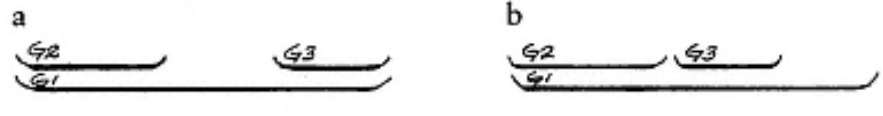
\includegraphics[scale=0.35]{gttm/GWFR_fig33.png}
	\end{center}
	\legend{Fonte: \cite{lerdahl1983generative} }
\end{figure}


\subsubsection{Regras de preferência para agrupamentos (GPRs)}

\begin{citacao}
\textbf{GPR1} “Evite analises com pequenos grupos, quanto menor menos preferível”.
\cite[ p.43]{lerdahl1983generative}
\end{citacao}

Segundo a GTTM, pequenos grupos geralmente não serão capazes de sozinhos estabelecer contextos. Uma pequena digressão: isto seria questionável em uma teoria que considerasse pequenos motivos como uma espécie de "objeto sonoro"\cite{guigue1995analise} , mas não é o caso desta abordagem, que está preocupada com uma camada exterior que supostamente é edificada por esta articulação contígua de grupos internos. A ideia de um pequeno motivo que irrompe esta superfície funcional linear como uma sonoridade \cite{guigue2012} articulada como entidade seria um complemento  interessante a ser pensando mais adiante.

\begin{citacao}
\textbf{GPR2 “(Proximidade)} – Considere uma sequencia de quatro notas [n1-n2-n3-n4], O restante sendo igual, a transição n2-n3 deve ser considerada uma fronteira de segmento se: \textbf{a) (Ligadura/Pausa)} o intervalo-temporal desde o final de n2 ao ínicio de n3 é menor do que desde final de n3 ao início de n4. \textbf{b) (Ponto-de-ataque)} o intervalo-temporal entre os pontos de ataque entre n2-n3 é maior do que entre n1-n2  e entre n3-n4. \cite[ p.45]{lerdahl1983generative}
\end{citacao}

Esta regra é centrada na busca por rupturas no fluxo dos motivos, isolando as frases pelos pontos de ataque fortes, ligaduras ou intervalos claros entre dois motivos.  

É notória a semelhança desta regra com o procedimento que aprendemos desde a alfabetização gramatical para a “separação de sílabas”\ - a procura de “respiros”\ das frases. É interessante também pensar a segmentação dos agrupamentos com analogias sobre a teoria da forma\cite{tenney1980temporal}.

%%%%%%%%%%%%%%%%%% elisao overlay gestalt
\begin{figure}[htb]
	\caption{\label{fig_grafico}Formalização visual dos problemas de elisão e sobreposição de camadas na GTTM. \cite[ p.69]{lerdahl1983generative}}
	\begin{center}
	    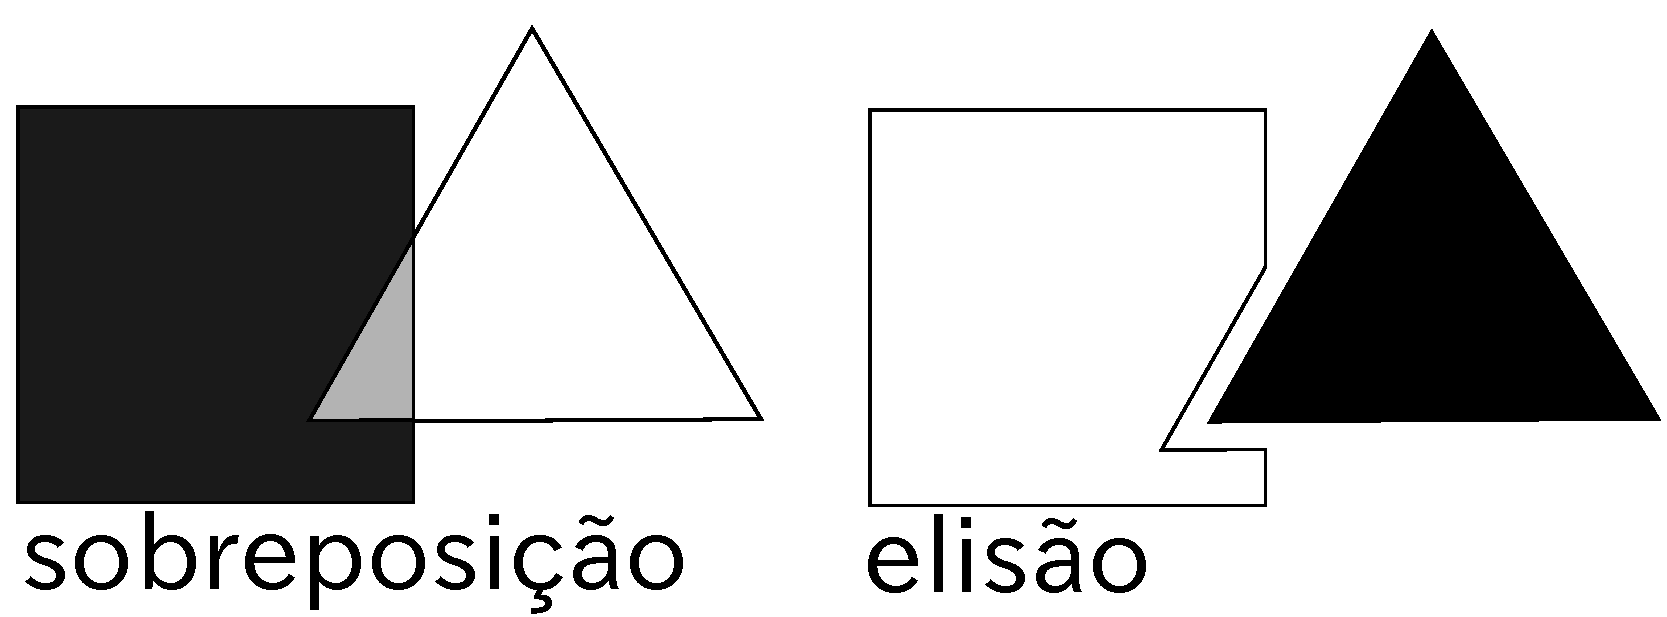
\includegraphics[scale=0.25]{gestalt/gestalt_elision_overlay.pdf}
	\end{center}
	\legend{Fonte: autor}
\end{figure}


\begin{citacao}
“Estes exemplos visuais parecem não ser apenas analogias triviais ao fenômeno musical. Como nas discussões de regras de preferência, a possibilidade de traçar paralelos entre os domínios auditivo e visual apontam a operação de processos fundamentais de da percepção e/ou cognição.” \cite{lerdahl1983generative} 
\end{citacao}

A busca de critérios para uma segmentação intuitiva destes “respiros” entre os motivos vai permear de alguma forma todo esforço da GTTM. 

Quanto a analogia com os critérios de segmentaçao da língua escrita e falada, percebemos na GTTM e sua revisão trabalhada por \citeonline{lerdahl2009genesis} um descrédito quanto ao fato que a música poderia simplesmente transpor metaforicamente as regras transformacionais da linguistica chomskiana, como por exemplo nas separações por classes gramaticais em complementos nominais e complementos verbais.  De fato para tal percurso seria necessário uma certa “licença poética” mais arbitrária.

\begin{citacao}
“O que a comparação atenta da linguagem verbal e da música nos ensinou, é que a significação em música não tem o mesmo estatuto que na linguagem.”\cite[ p.9]{nattiez2004modelos}
\end{citacao}

Por outro lado, obviamente seria preciso pensar todas as características para além do aparecimento temporal dos eventos.

Além do “respiro”, passamos a levar em consideração alguns critérios de modificação do som como altura, força do ataque, gestual da articulação e o envelope de duração nas emendas dos segmentos. No entanto iremos perceber que recursivimente a teoria vai demandando definições mais precisas para cada novo critério que enumera. Por exemplo: como definir "articulação"? Que critérios utilizar nas medidas intervalares?


\begin{citacao}
\textbf{GPR3 (Mudança)} Considere uma sequencia de notas [n1-n2], a transição [n2-n3] deve ser ouvida como um grupo de fronteira se marcado por: \textbf{a) registro} – a transição n2-n3 envolve uma maior distância intervalar de que entre n1-n2 ou n3-n4, \textbf{b) dinâmica} - a transição n2-n3 envolve uma mudança dinâmica maior de que entre n1-n2 ou n3-n4, \textbf{c) articulação} - a transição n2-n3 envolve uma mudança de articulação maior de que entre n1-n2 ou n3-n4, \textbf{d) duração} - há diferença de durações  entr n2-n3 enquanto n1-n2 ou n3-n4 permanecem com durações similares,
\cite{lerdahl1983generative}
\end{citacao}


Ilustramos algumas destas regras demonstrando como podem ser observadas em uma estrutura \textit{chord-seq} da linguagem \textit{Open Music}.\footnote{As ferramentas computacionais utilizadas neste trabalho são explicadas em detalhes na \autoref{computacional}. }


\begin{figure}[htb]
	\caption{\label{fig_grafico}Open Music}
	\begin{center}
	    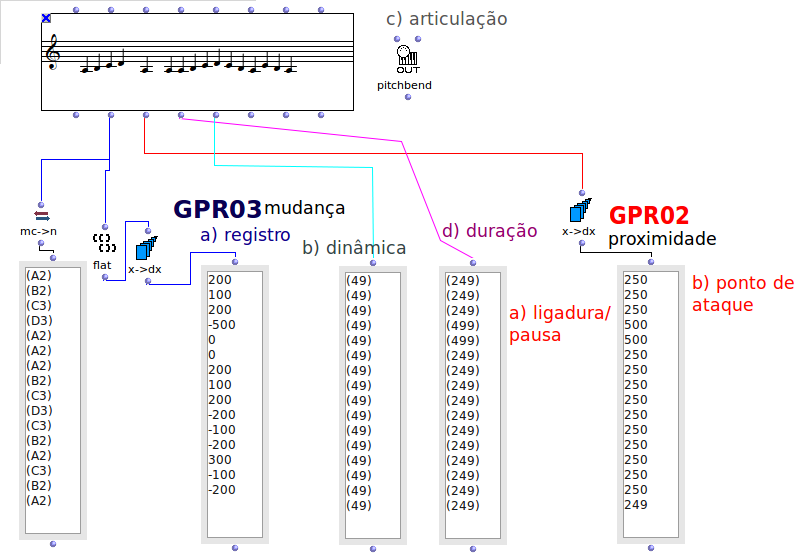
\includegraphics[scale=0.6]{mikro/OM_gttm_GPR02-03.png}
	\end{center}
	\legend{Fonte: autor }
\end{figure}


As regras seguintes especializam as GPRs anteriores, filtrando agrupamentos que tendem a ficar em níveis mais frasais do que os pequenos motivos que deverão conter em sua composição:

\begin{citacao}
\textbf{GPR4 (Intensificação)} Onde os efeitos dos GPR 2 e 3 são relativamente mais pronunciados, um grupo de nível mais largo deve ser localizado. \textbf{GPR5 (Simetria)} Prefira análise de agrupamentos com a abordagem mais próxima da subdivisão de grupos em partes de duração iguais. \textbf{GPR6 (Paralelismo)} Onde dois ou mais segmentos musicais podem ser construídos em paralelo, eles preferivelmente formam partes paralelas dos grupos \textbf{GPR7 (Estabilidade de prolongacional e de intervalo-tempo )} Prefira uma estrutura de agrupamento em um intervalo-tempo tempo mais estável e/ou reduções prolongacionais.
\cite[ pg.46-52]{lerdahl1983generative}
\end{citacao}


\subsection{Estrutura Métrica}

Antes de entrar na taxonomia das regras de boa formação métrica convém entender o que a GTTM coloca como acento. Há uma categorização que divide os acentos em fenomenológico , estrutural e métrico.

Por fenomenológicos os autores entendem acentos que são causados por eventos marcantes e destacados da superfície musical como pontos extremos no contorno melódico, stress ou relaxamento súbito nas articulações ou pontos de tensão inesperada na harmonia, estruturais seriam acentos bem marcados pelas cadências de progressões harmônicas mais marcantes e esperadas.

Métricos são os acentos que estão no pulso intuitivo da superfície musical, nos tempos fortes e síncopas, e que de alguma maneira reforçam uma marcação rítmica esperada pela peridiocidade dos eventos. 

Os autores não associam diretamente este tipo de acento a uma declaração de assinatura de compasso na escritura da peça, mas sugerem que de alguma maneira este tipo de acento é justamente uma relação de afirmação ou negação dessa possibilidade de haver uma peridiocidade forte nos eventos, que a escritura tentaria prever. 


%%%%%%%%%%%%%%%%%% ritmica gttm
\begin{figure}[htb]
	\caption{\label{fig_grafico}Notação analítica proposta pela GTTM que marca uma hierarquia das batidas por subdivisões de pulsos}
	\begin{center}
	    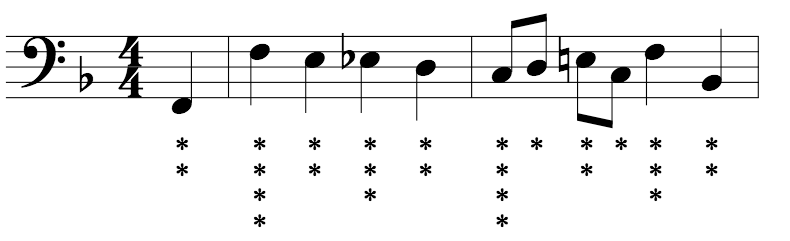
\includegraphics[scale=0.45]{gttm/GTTM-m21-metes.png}
	\end{center}
	\legend{Fonte: Documentação da biblioteca python music21}
\end{figure}


As regras de boa formação métrica na GTTM estabelecem as condições mínimas para que o efeito de periodicidade aconteça.  Observa-se que se por uma lado a escrita tradicional com seus compassos e assinaturas serve como um ponto de partida e apoio para contagem de batidas baseadas nas subdivisões das figuras métricas ela também é fator limitador na redução dos intervalos-temporais. Este problema aparece na GTTM como “apagamento métrico”\cite[pg.101]{lerdahl1983generative}, algo similar a colisões e elisões vistas nos agrupamentos. 

Não é por acaso que a partir do século XX a escrita com mudanças constantes de assinatura de compasso chega em um ponto, após o serialismo integral principalmente, em que é proposta a abolição da assinatura ou barra de compassos num extremo e no outro extremo uma complexidade tão alta na subdivisão de quiálteras que ficam totalmente arbitrárias e subentendidas na notação uma indução ao improviso do interprete.

Voltando às regras, assim como no agrupamento, na métrica também temos as regras de boa formação (WFRs - “Well Formed Rules”) para os casos mais gerais e em seguida atemos as regras de preferência (PRs - “Preference rules”), hierarquizando as decisões.

\begin{citacao}
\textbf{MWFR 1 }"Todo ponto de ataque deve estar associado a uma batida de nível métrico menor presente naquele ponto da peça",  
\textbf{MWFR 2} "Toda batida em dado nível deve também ser uma batida em níveis menores daquele presente ponto da peça", 
\textbf{MWFR 3} "A cada nível métrico, batidas fortes são espaçados por uma separação de duas ou três batidas" 
\textbf{MWFR 4} "O tátil e o material imediatamente mais largo devem consistir de batidas igualmente espaçadas através da peça. No nível subtátil, batidas fracas devem estar igualmente espaçadas entre as batidas fortes que os cercam." 
 \cite{lerdahl1983generative}
\end{citacao} 

\subsubsection{Regras de preferência métrica (MPFRs) } 

O conjunto de regras de preferência métrica estabelece conflitos que inevitavelmente precisariam ser hierarquizados conforme o contexto, e da mesma maneira que as regras gerais de agrupamento, são dependentes de maior critério na definição dos eventos de alturas, cadências e articulações.

\begin{citacao}
\textbf{MPFR1 (Paralelismo) }"Onde dois ou mais grupos ou partes de grupos podem ser construídos em paralelo, eles preferivelmente recebem uma estrutura métrica paralela" 
\textbf{MPFR2 (Batida forte adiantada)} "Prefira raramente uma estrutura métrica onde a batida mais forte em um grupo aparece relativamente adiantada no grupo" 
\textbf{MPFR3 (Evento)} "Prefira uma estrutura material onde as batidas do nível Li coincidem com a inserção de eventos de altura nas batidas fortes de Li" 
\textbf{MPFR4 (Tensão)} "Prefira uma estrutura métrica onde as batidas do nível Li são tensionadas com as batidas fortes de Li" 
\end{citacao}

\begin{citacao}
\textbf{MPFR5 (Duração)} "Prefira uma estrutura métrica onde batidas relativamente fortes ocorrem na inserção de também relativamente longos: 
\textbf{a)} evento de altura 
\textbf{b)} duração de dinâmica 
\textbf{c)} ligadura 
\textbf{d)} padrão de articulação 
\textbf{e)} duração de um pitch em níveis relevantes da redução intervalo-temporal 
\textbf{f)} duração da harmonia em níveis relevantes  da reduação intervalo-temporal (ritmo harmônico )
\end{citacao}

\begin{citacao}
\textbf{MPFR6 (Baixo)} "Prefira um baixo metricamente estável" 
\textbf{MPFR7 (Cadência)} "Prefira fortemente uma estrutura métrica onde as cadências são metricamente estáveis; ou seja, evite fortemente violações das regras de preferência locais que possuem cadências" 
\textbf{MPFR8 (Suspensão)} "Prefira fortemente uma estrutura métrica onde a suspensão é uma batida mais forte que a resolução" 
\textbf{MPFR9 (Interação intervalo-temporal)} "Prefira uma análise metrica que minimize o conflito na redução do intervalo-temporal" 
\textbf{MPFR10 (Regulação Binária)} "Prefira estruturas métricas em que em cada nível toda a outra batida seja forte" 
 \cite{lerdahl1983generative}
\end{citacao}



\section{Segmentação temporal de eventos cadenciais e a redução prolongacional na GTTM}


É importante destacar a partir daqui que as continuidades e derivações da pesquisa iniciada pelo GTTM tiveram que buscar fórmulas mais rigorosas em pesquisas quantitativas sobre "cognição das alturas musicais"\cite{krumhansl1990cognitive} nos níveis de interação entre as camadas melódico-harmônicas com os agrupamentos métrico-rítmicos para sustentar seus argumentos sobre as preferências condicionadas do tal "ouvinte experiente"\cite[pg. 118]{lerdahl1983generative} como fator organizador da teoria. 

As regras de redução prolongacional, similares aos resumos cadenciais shenkerianos que segmentam os eventos melódico-harmônicos, são dependentes daquilo que a GTTM chama de intervalo-temporal ("time span") - regras de preferência determinadas por fatores internos da superfície musical: proximidade de uma tônica, modulação de regiões funcionais de tonalidade, âmbito de registro de oitava, paralelismo motívico e toda uma suposta hierarquia destas interações. No entanto estes apontamentos foram desde então criticados por sua arbitrariedade indutiva.\footnote{ c.f. "Pontos típicos da crítica"\ da GTTM em \cite[pg. 35]{hansen2011legacy} }

O próprio \citeonline{lerdahl2009genesis} afirma em sua revisão da GTTM:


\begin{citacao}
O princípio de interação talvez ainda seja muito técnico para ser testado empiricamente neste ponto; mas em seu contexto mais amplo, a percepção hierárquica das estruturas de alturas é um assunto de interesse considerável para a psicologia da música.\textbf{ O componente de prolongamento da GTTM de qualquer modo, apresenta dificuldades a este respeito.}\cite[p. 191]{lerdahl2009genesis}\footnote{ The interaction principle itself may still be too technical to be tested empirically at this point, but its larger
context, the perception of hierarchical pitch structures, is a topic of considerable interest to music psychology. GTTM’s prolongational component, however, presents
difficulties in this regard. \cite[p. 191]{lerdahl2009genesis}}
\end{citacao}



Posteriormente ao GTTM, Lerdahl investe esforços no desenvolvimento da teoria de espaço tonal\cite{lerdahl1988tps}. Esta teoria foi fortemente baseada nas pesquisas de quantificação das condições para estabilidade da percepção de contextos tonais argumentada por Carol Krumhansl em seu artigo \textit{"Perceptual structures of tonal music"}\cite{krumhansl1983perceptual} e fundamentada em mais profundidade no livro \textit{"Cognitive structures of pitch"}\cite{krumhansl1990cognitive}. Como veremos mais adiante este trabalho também influenciou os algoritmos de harmonia e tonalidade de David Temperley em seu \textit{"Cognition of Basic Musical Structures"}\cite{temperley2001cognition}. 


Mais recentemente, Lerdahl atualiza sua teoria do espeço tonal\cite{lerdahl2001tonal} buscando alguns argumentos novos sobre transformações cromáticas algébricas fundamentadas pela corrente musicológica \textit{"Neo-Riemaniana"}\cite{cohn1998introduction,lewin2007generalized} e escreve com Krumhansl um artigo chamado \textit{"Modeling Tonal Tension"}\cite{2007lerdahl-krumhansl} a fim de legitimar sua teoria através de testes cognitivos com uma audiência.

\begin{citacao}
A ideia é que a distância cognitiva de um evento de um ponto dado de referência mede a instabilidade do evento em relação a este ponto de referência. Na suposição que o ouvinte inconscientemente busca uma interpretação mais estável de uma passagem musical, o principio TPS ["Espaço de Alturas Tonais"] do menor caminho seleciona eventos revelando as menores distâncias disponíveis para superordenar eventos em cada estágio da redução prolongacional.\cite[p. 191]{lerdahl2009genesis}\footnote{The idea is that the cognitive distance of an event from a given reference point measures the instability of that
event in relation to the reference point. On the assumption that the listener unconsciously seeks the most stable construal of a musical passage, TPS’s principle of
the shortest path selects events yielding the smallest available distances from superordinate events at each stage of prolongational reduction. \cite[p. 191]{lerdahl2009genesis}}
\end{citacao}

%%%%%%%%%%%%%%%%%% tonal pitch space
\begin{figure}[!h]
	\caption{\label{fig_grafico}Extensão das regras de GTTM na obra “Tonal Pitch Space” propostas por \citeonline{lerdahl2009genesis} }
	\begin{center}
	    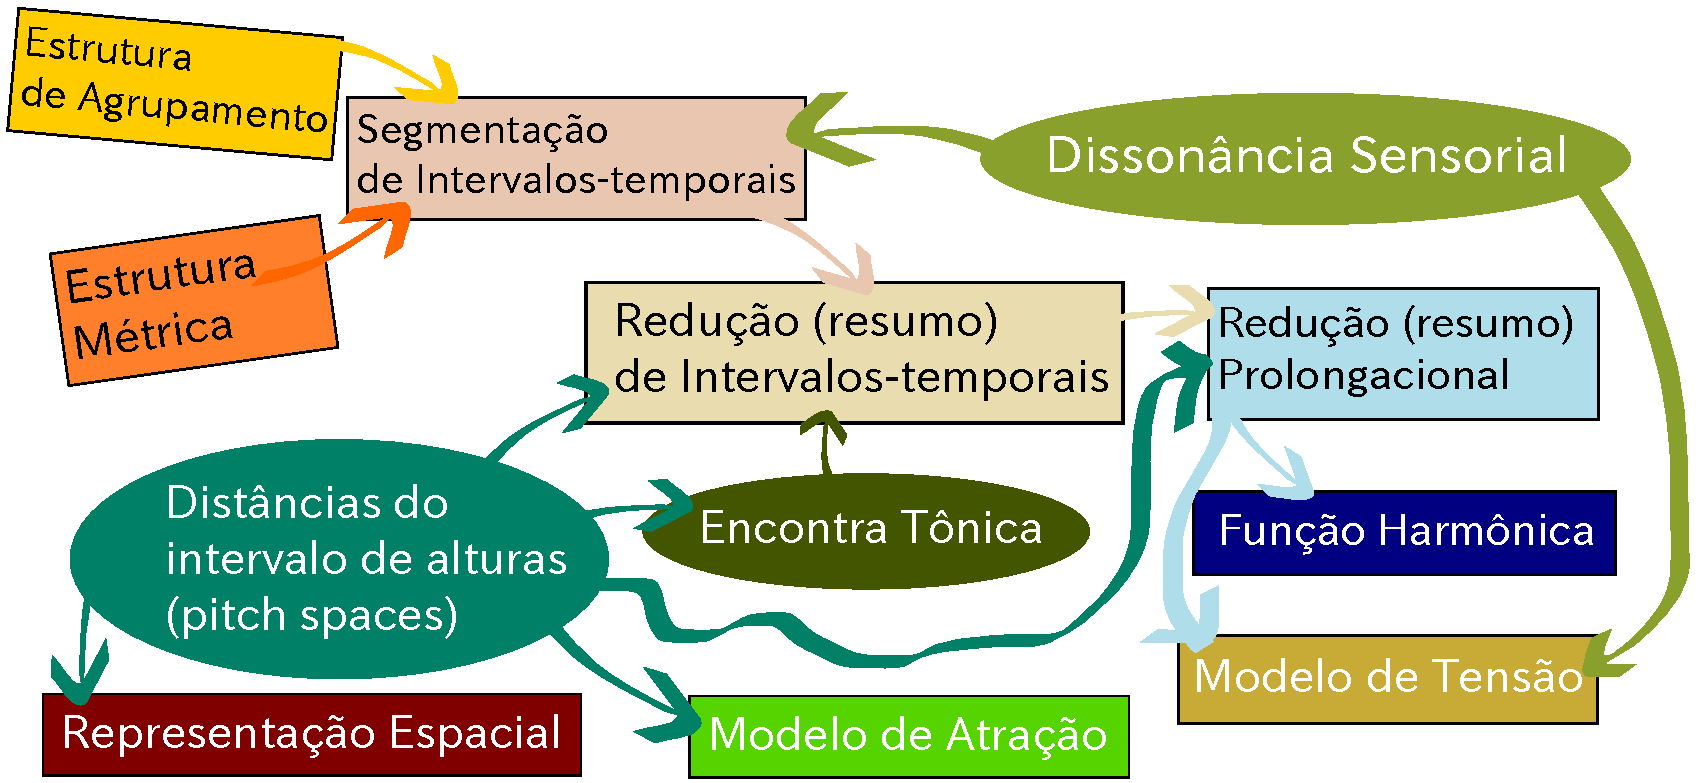
\includegraphics[scale=0.5]{gttm/GTTM_TPS_rules.pdf}
	\end{center}
	\legend{Fonte: \cite[ tradução do autor.]{lerdahl2009genesis} }
\end{figure}


Considerando esta atualização da teoria, optamos por não entrar em detalhes destes dois escopos mais frágeis da GTTM e focamos diretamente em derivações posteriores que os problematizam em outros termos. Tomamos dos estudos de Lerdahl posteriores à GTTM  por enquanto apenas seu conceito de tensão e estabilidade desenvolvido em sua "teoria do espaço tonal"("Tonal Pitch Space", doravante referida como TPS) na próxima sessão. Em seguida apresentamos uma alternativa derivada da GTTM, elaborada por David Temperley e implementada computacionalmente em seu trabalho "Cognition of Basic Musical Structures"\cite{temperley2001cognition}.


\subsubsection{Calculando a tensão e o espaço das alturas tonais (TPS) }


Para a segmentação prolongacional da GTTM, \citeonline{lerdahl1983generative} já argumentavam regras de formação que determinariam ramificações semelhantes às usadas por Chomsky\cite{chomsky1957syntactic} para construir as implicações de um segmento sobre outro. Como nas frases escritas, a ideia deriva da constatação de que adjetivos qualificam substantivos, pronomes conjugam verbos e assim por diante. Estas estruturas sintáticas determinam uma boa-formação da frase, de maneira que, mesmo antes de inferirmos significado nesta, temos uma estrutura onde as funções estão bem definidas. A troca de um verbo por outro, por exemplo, contanto que conjugados na mesma pessoa do sujeito da frase, muda seu sentido - mas não sua sintaxe.

\begin{figure}[!h]
	\caption{\label{fig_grafico}"Ideias verdes descoloridas dormem furiosamente"\cite{chomsky1957syntactic}}
	\begin{center}
	    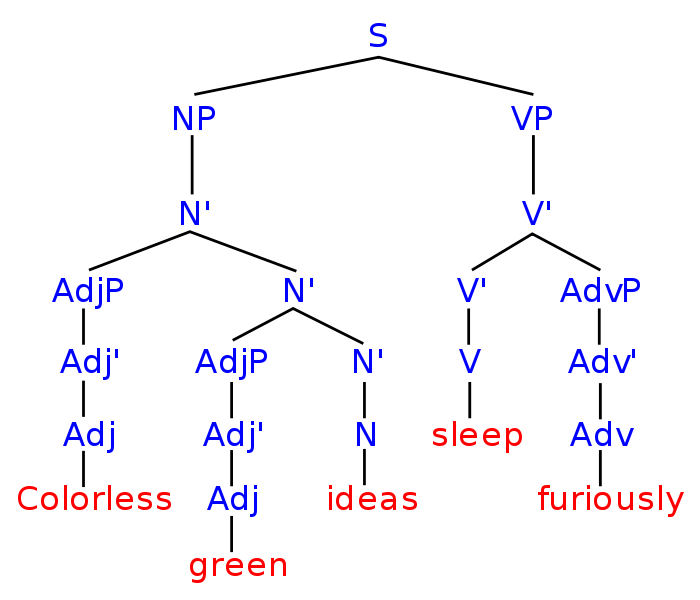
\includegraphics[scale=0.45]{gttm/colorless.png}
	\end{center}
	\legend{Fonte: wikimedia.org}
\end{figure}

A frase \textbf{"Ideias verdes descoloridas dormem furiosamente"} é usada por \citeonline{chomsky1957syntactic} em sua argumentação sobre a construção de uma frase onde a ordem correta e implicação funcional das palavras determina sentido mas não uma semântica estrita. Mesmo a tradução para português já revela uma problemática básica para os algoritmos de tradutores textuais - se traduzirmos literalmente palavra por palavra não teremos uma frase bem construída: \textbf{"Descoloridas verde ideias dormem furiosamente"}.

\pagebreak
%%%%%%%%%%%%%%%%%% tree
\begin{figure}[!h]
	\caption{\label{fig_grafico}A analogia de um segmento musical implicando ou sendo implicado por outro é usada na GTTM.}
	\begin{center}
	    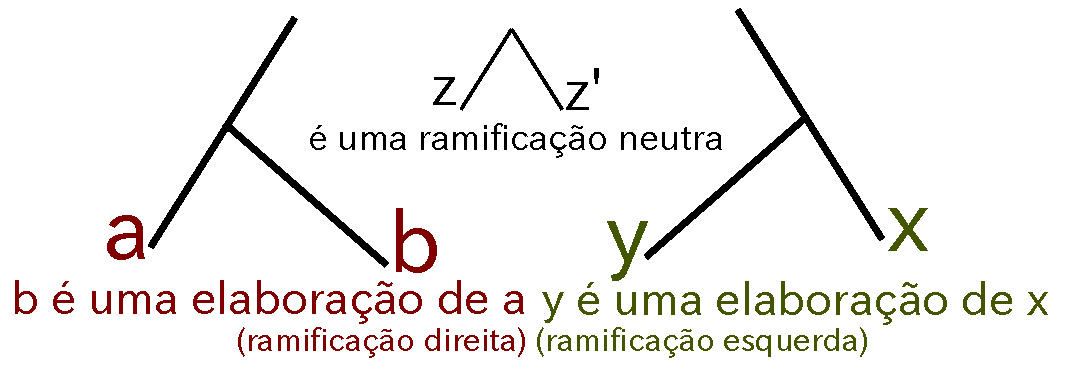
\includegraphics[scale=0.4]{gttm/ramificacoes_arvore.pdf}
	\end{center}
	\legend{Fonte: autor }
\end{figure}


\begin{figure}[!h]
	\caption{\label{fig_grafico}Notação em árvore proposta pela GTTM aplicada na melodia inicial de Mikrokosmos 113 de Bártok.}
	\begin{center}
	    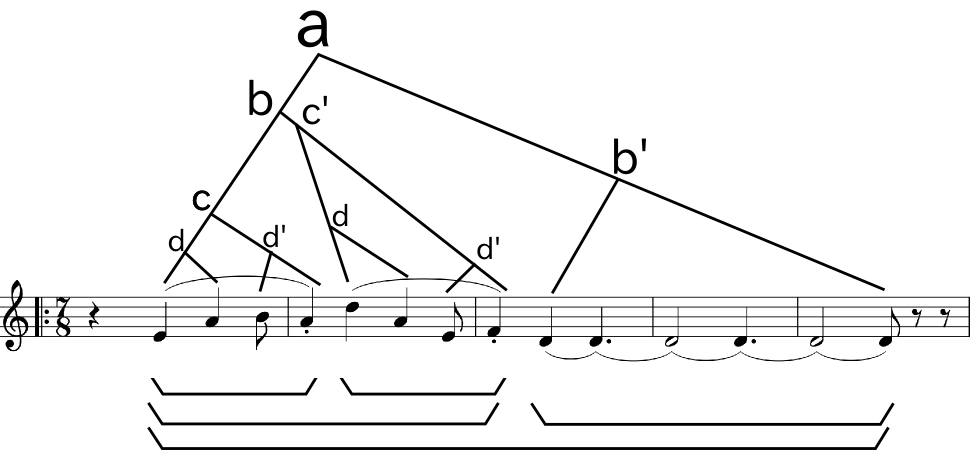
\includegraphics[scale=0.4]{mikro/mikro113_GTTM_tree.png}
	\end{center}
	\legend{Fonte: autor}
\end{figure} 

\pagebreak
Na GTTM\cite[pg. 182]{lerdahl1983generative} é apresentada uma notação com círculos brancos para prolongamentos fortes e pretos para prolongamentos fracos. No entanto naquele momento ainda não havia uma argumento quantitativo rigoroso para medir estas forças.

%%%%%%%%%%%%%%%%%% tree
\begin{figure}[!h]
	\caption{\label{fig_grafico}Forças tonais nos prolongamentos revistas por Fred \citeonline{lerdahl1988tps} }
	\begin{center}
	    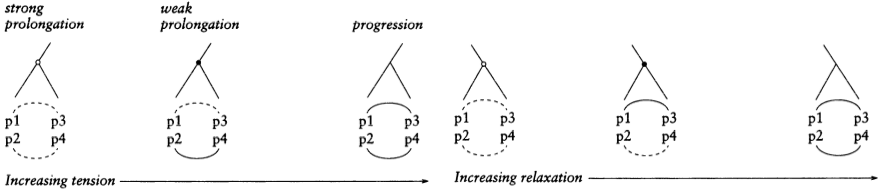
\includegraphics[scale=0.5]{lerdahl/prolongation_calculating.png}
	\end{center}
	\legend{Fonte: \cite[p. 322]{lerdahl1996calculating} }
\end{figure}


Em seus artigos "Tonal Pitch Space"\cite{lerdahl1988tps} e "Calculating Tonal Tension"\cite{lerdahl1996calculating} elabora com mais rigor o desenvolvimento de um critério para determinar numericamente estas forças e decidir prolongamentos que prevalecem nas reduções ou argumentar momentos de mudança de contexto tonal. 


A fórmula determina um peso para a transformação da condução de vozes para arbitrar uma escala de valores numéricos entre os adjetivo "forte"\ e "fraco"\ que permite especular uma computabilidade destes movimentos de tensão e relaxamento.

\pagebreak
Lerdahl utiliza o modelo de espaço derivado de \citeonline{deutsch1981internal}, que hierarquiza as alturas em níveis cromático, diatônico, triádico, quintas e oitavas. Distribui as alturas normalizadas em grupos de classe de alturas, desconsiderando o registro de oitava, para em seguida comparar as regiões.

%%%%%%%%%%%%%%%%%% tree
\begin{figure}[!h]
	\caption{\label{fig_grafico}Espaço tonal diatônico proposto por Fred \citeonline{lerdahl1988tps} }
	\begin{center}
	    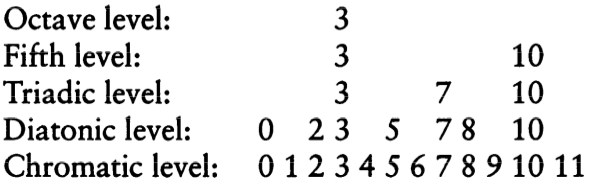
\includegraphics[scale=0.4]{lerdahl/diatonic_pitchspace_p322.png}
	\end{center}
	\legend{Fonte: \cite[p. 322]{lerdahl1996calculating} }
\end{figure}

O exemplo usado é o início da Sonata K.282 de Mozart, demonstrando as tonalidades a partir do I grau de Eb maior. 

$ Eb:I\left\{
  \begin{array}{l l}
    Nível\;Oitava:[3]\to[Eb]\to Tonalidade\\
    Nível\;Quinta:[3,10]\to[Eb,Bb]\to Dominante\\
    Nível\;Tríadico:[3,7,10]\to[Eb,G,Bb]\to Tríade\;Maior \\
    Nível\;Diatônico:[3,5,7,10,0,2] \to Escala\;de\;Eb\; Maior \\
    Nível\;Diatônico:[0...11] \to Sequencia\;cromática\;completa \\
    
  \end{array} \right.
$

Para decidir quais graus do prolongamento são mais fortes a ponto de permanecerem em reduções e figurarem como tensão e relaxamento, \citeonline[pg.232]{lerdahl1996calculating} utiliza a fórmula: 
$
distância(x \to y) = i+j+k \\
$


$ onde\left\{
  \begin{array}{l l}
i=passos\;entre\;tonalidades\;por\;ciclo\;de\;quintas \\
j=passos\;entre\;acordes\;por\;ciclo\;de\;quintas \\
k=graus\;cromáticos\;em\;comum \\

  \end{array} \right.
$

%%%%%%%%%%%%%%%%%% tree
\begin{figure}[!h]
	\caption{\label{fig_grafico}Prolongamentos na Sinfonia K.238 }
	\begin{center}
	    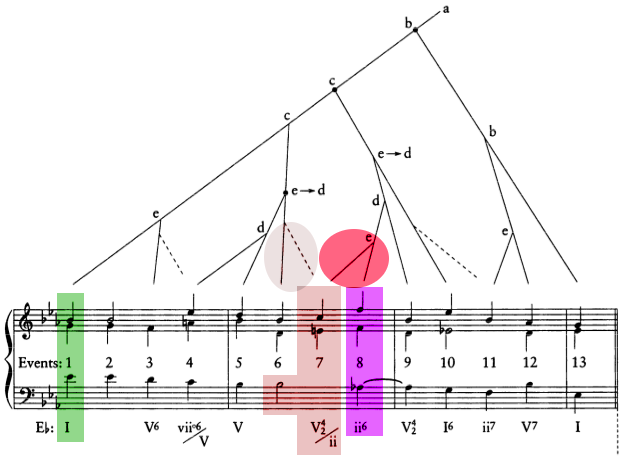
\includegraphics[scale=0.6]{lerdahl/calculating_prolongamento.png}
	\end{center}
	\legend{Fonte: \cite[p. 323]{lerdahl1996calculating} }
\end{figure}

Lerdahl numera as cadências e determina algumas preferências para a decisão de quais segmentos são tensão e relaxamento nos prologamentos, através da sua fórmula para medida das distâncias.

%%%%%%%%%%%%%%%%%% tree
\begin{figure}[!h]
	\caption{\label{fig_grafico}Exemplo de aplicação da fórmula das distâncias }
	\begin{center}
	    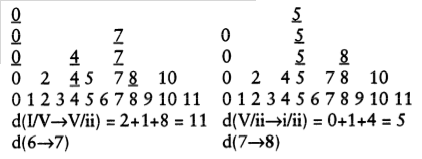
\includegraphics[scale=0.7]{lerdahl/pitchspace-K282.png}
	\end{center}
	\legend{Fonte: \cite[p. 323]{lerdahl1996calculating} }
\end{figure}



No caso $(6 \to 7)$ temos \textbf{2} passos pelo ciclo de quintas para chegar de $(V \to ii)$, \textbf{1} passo para chegar de $(I \to V)$ e 8 graus cromáticos em comum. Uma distancia de "tensão tonal"\ igual a \textbf{11}.\pagebreak

No caso $(7 \to 8)$ temos \textbf{1} passos pelo ciclo de quintas para chegar de $(V \to i)$, \textbf{0} passos para chegar de $(ii \to ii)$ e 4 graus cromáticos em comum. Uma distancia de "tensão tonal"\ igual a \textbf{5}.

Toma-se o menor como equivalente a "menor distancia"\ na tensão tonal, portanto prevalece o movimento $(7 \to 8)$. 



\section{Cognição das estruturas musicais básicas (CBMS)}

A teoria elaborada por David \citeonline{temperley2001cognition} em seu livro \textit{"Cognition of Basic Musical Structures"}\footnote{Doravante tratado por CBMS. } foi declaradamente inspirada na GTTM. Seu esquema de enumeração de regras \textit{bem formadas} e regras \textit{de preferência} é tão similar que pode ser considerado uma tentantiva de continuidade desta.

Temperley divide as regras em seis grupos: \textbf{estrutura métrica, frase melódica, estrutura contrapontual, solfejo enarmônico das classes de altura tonais, estrutura harmônica, estrutura de tonalidade.}

As regras de estrutura métrica são bastante similares e as regras de frase melódica e estrutura contrapontual são uma proposta próxima das regras de agrupamento da GTTM, porém levando em conta algumas ideias para interação polifônica e determinando métodos para pensar contorno melódico e o fluxo das vozes. 

Decidimos iniciar o percurso pelas regras da CBMS com dois grupos de regras que parecem indispensáveis para pensar todas as outras, e que parece mais deficiente na GTTM: o solfejo enarmônico das classes de altura tonais e a estrutura de tonalidade. 


\subsubsection{Solfejo Enarmônico das Classes de Alturas Tonais}
\label{solfejo}
A questão do solfejo enarmônico é central para a implementação algorítmica dos seis sistemas de regras propostos por Temperley.

A CBMS parte de uma reflexão sobre representações geométricas do ciclo de quintas, concluindo que representações cíclicas e modulares do ciclo ("Neutral Pitch Class") não são suficientes para o que chama "Tonal Pitch Class", uma representação que dê conta dos contextos funcionais que diferenciam as enarmonias conforme o seu papel em determinado contexto: nota sensível, nota de passagem, modulação para tonalidade relativa, resolução de dominante, etc.\footnote{Para além de declarações de tonalidade na escrita tradicional de armaduras de clave, Temperley leva em consideração aquilo que há de autoral na ortografia\cite[p.123]{temperley2001cognition}  dos compositores e que poderia confirmar a função do cromatismos dentro do discurso tonal cognoscível para o sistema argumentado pelas CBMS.}

\begin{figure}[!h]
	\caption{\label{fig_grafico}Ciclo de dominantes e subdominantes em modo circular }
	\begin{center}
	    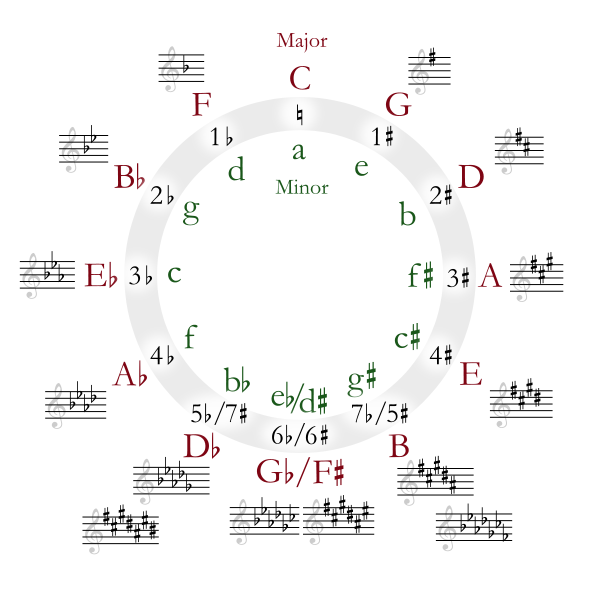
\includegraphics[scale=0.4]{CBMS/quintas.png}
	\end{center}
	\legend{Fonte: wikisource.org }
\end{figure}


Considerando a representação geométrica circular das classes de nota problemática para enarmonia, por ser cíclica e não representar o deslocamento de intervalos dentro da distância superior a um âmbito limitado de oitava, a  CBMS propõe uma medida para esta denominação baseada no que chama de "linha de quintas".

O argumento é de que a linha sugere possíveis cromatismos através de uma provável modulação desejada para mover-se até tonalidades vizinhas.


\begin{figure}[!h]
	\caption{\label{fig_grafico}Escala de Dó maior na linha enarmônica das quintas proposta por Temperley. }
	\begin{center}
	    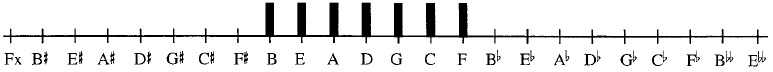
\includegraphics[scale=0.6]{CBMS/jonico_lineoffifths.png}
	\end{center}
	\legend{Fonte: \cite[pg. 127]{temperley2001cognition} }
\end{figure}

\pagebreak
Nas regras de preferência para o Solfejo enarmônico  CBMS problematiza o que chama de "Centro de Gravidade Tonal"\footnote{(COG)-"Center of gravity"\cite[ p.125]{temperley2001cognition}}.

\begin{figure}[!h]
	\caption{\label{fig_grafico}Escala de Dó maior - Ré como centro de gravidade. }
	\begin{center}
	    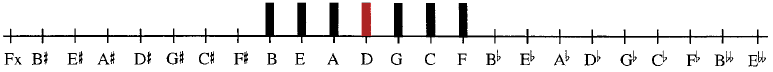
\includegraphics[scale=0.6]{CBMS/COG_re_lineoffifths.png}
	\end{center}
	\legend{Fonte: \cite[pg. 127]{temperley2001cognition} }
\end{figure}
\pagebreak
Considera-se que cada centro de gravidade vai ficando mais complexo a cada modulação de tonalidade. A regra de preferência da variância das alturas\footnote{"Tonal Pitch Rule 1"\ - (TPR1)\cite[ p.125]{temperley2001cognition}} determina a aproximação onde, por exemplo, para a escala de Dó maior teremos o centro em Ré.

Mais adiante em uma aplicação proposta para a análise da influência do modalismo no rock, Temperley propõe uma ideia que chama de "supermodo", uma combinação de modos vizinhos, expandindo o espaço tonal para um campo estendido onde as notas cromáticas teriam funções de afirmar os modos.

\begin{figure}[!h]
	\caption{\label{fig_grafico}Escalas modais na linha enarmônica das quintas proposta por Temperley e o supermodo resultante de sua combinação. }
	\begin{center}
	    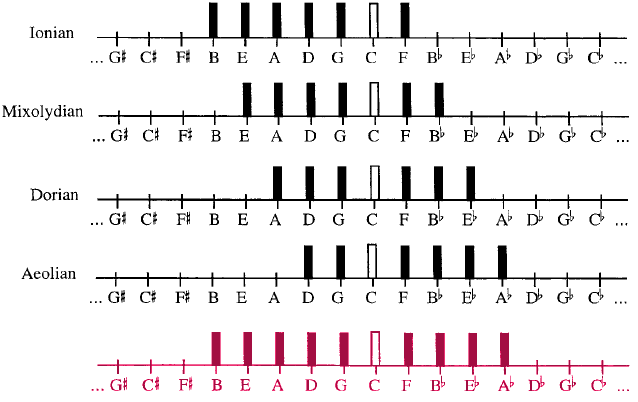
\includegraphics[scale=0.6]{CBMS/modosrockgregos_temperley.png}
	\end{center}
	\legend{Fonte: \cite[pg. 260]{temperley2001cognition} }
\end{figure}


As regras de variância na condução de vozes\footnote{"Tonal Pitch Rule 2" - (TPR2)\cite[ p.129]{temperley2001cognition}} determinam critérios para considerar as passagens cromáticas dentro da condução de vozes, já que neste caso é preciso uma "nota de passagem"\ que não está como pivô de modulação ou sensível de resolução mas como um ornamento de passagem cromática. A CBMS propõe que se um evento está distante do centro de gravidade neste contexto deve portanto estar a no mínimo cinco passos da classe de altura do evento relacionado \cite[ p.130]{temperley1997algorithm}.

A última regra de preferência para o solfejo harmônico trata do reconhecimento de notas que estão figurando funcionalmente em acordes, determinando contexto cadencial.\footnote{"Tonal Pitch Rule 3" - (TPR3)\cite[ p.131]{temperley2001cognition}}

A regra anterior expõe um caso onde claramente não apenas o contexto é determinado pela escolha da relação individual entre as alturas  mas a identidade destas alturas é determinada pelo contexto harmônico. 

A CBMS estabelece regras específicas para inferir contexto harmônico, mas em nossa abordagem preferimos antes explorar sua argumentação para a estrutura de tonalidade, buscando as raízes dos argumentos que sustentam tal teoria harmônica. 


\pagebreak
\subsubsection{Algoritmo dos Perfis de Tonalidade}
\label{perfiltonal}

Temperley problematiza os algoritmos de busca por tonalidade lembrando que identificar um solfejo de notas em uma passagem melódica não será suficiente se não soubermos qual o contexto de tonalidade da passagem\cite[p.167]{temperley2001cognition}.

Para isto inicia uma busca por um estudo comparado entre algumas abordagens da percepção de tonalidade, pela psicologia cognitivista da música. \cite{cuddy1979melody,brown1994musical,deutsch1981internal,longuet1971interpreting}

Decide focar no algoritmo de "Krumhansl-Schmuckler"\footnote{c.f. implementação em \url{http://web.mit.edu/music21/doc/moduleReference/moduleAnalysisDiscrete.html\#music21.analysis.discrete.KrumhanslSchmuckler}. Acesso em 10 de julho de 2014.}     
surgido da pesquisa de Carol \citeonline{krumhansl1983perceptual} e aprofundado em seu "Cognitive foundations of musical pitch"\cite{krumhansl1990cognitive}.


\begin{figure}[!h]
	\caption{\label{fig_grafico}Perfis de tonalidade propostos por Carol \citeonline{krumhansl1983perceptual} - comparativo entre tonalidades próximas e distantes. }
	\begin{center}
	    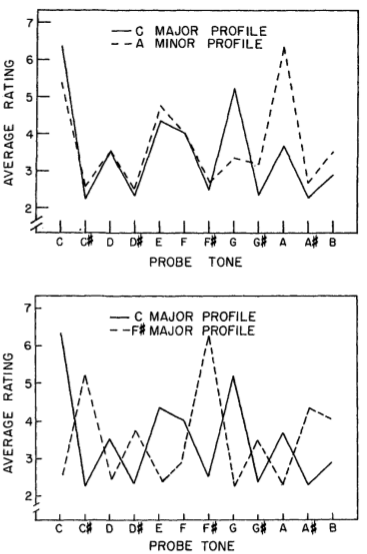
\includegraphics[scale=0.63]{CBMS/probeones_krumhansl_p36.png}
	\end{center}
	\legend{Fonte: \cite[pg. 36]{krumhansl1990cognitive} }
\end{figure}

Krumhansl argumenta sobre o que chama "perfis-tonais", histogramas que servem como uma referência para calculo estatístico a partir de uma amostra de ouvintes pesquisados sobre a tendência a "adaptar"\cite[p.173]{temperley2001cognition} notas de uma escala cromática como ornamentos dentro de um determinado contexto tonal.


\begin{figure}[!h]
	\caption{\label{fig_grafico}Perfis de tonalidade propostos por Carol \citeonline{krumhansl1990cognitive} - histograma demonstrado por \citeonline{temperley2001cognition}. }
	\begin{center}
	    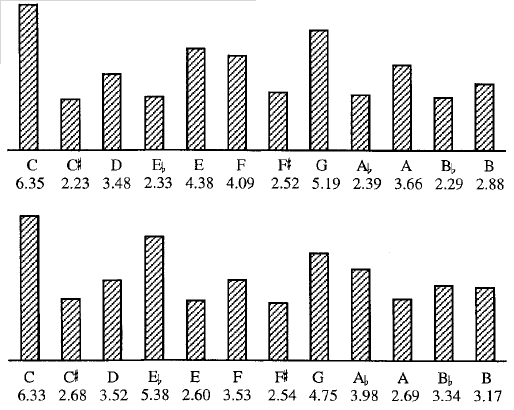
\includegraphics[scale=0.6]{CBMS/krumhansl_temperley_p174.png}
	\end{center}
	\legend{Fonte: \cite[pg. 174]{temperley2001cognition} }
\end{figure}


A fórmula funciona da seguinte maneira\footnote{c.f. uma prova real detalhada da fórmula original em \cite[p.37]{krumhansl1990cognitive} }:


$ \left\{
  \begin{array}{l l}
x = valores\;individuais\;do\;histograma\;original \\
\overline{x} = media\;de\;todos\;valores\;do\;histograma\;original \\
y = valores\;de\;um\;histograma\;a\;ser\;comparado - retirado\;de\;trecho\;musical \\
\overline{y} = media\;de\;todos\;os\;valores\;do\;histograma\;usado\;em\;y \\
    
  \end{array} \right.
$


\scalebox{2}{%
$
r= 
\frac{\sum{(x-\overline{x})(y-\overline{y})}}
{\sqrt{ \sum{ (x-\overline{x})^2 } \sum{ (y-\overline{y})^2 } } }
$
}
\linebreak
\linebreak
A escala cromática tem um padrão para o contexto de Dó maior e Dó menor, que para ser transposto para outras tonalidades bastando mover a ordem das alturas (por exemplo em Dó sustenido maior este passa a valer 6.35, Ré passa a valer 2.23 e assim por diante).
\pagebreak

Temperley propõe uma atualizações neste algoritmo\cite[pg.173-182]{temperley2001cognition}\footnote{c.f. implementação na biblioteca music21 em \url{http://web.mit.edu/music21/doc/moduleReference/moduleAnalysisDiscrete.html?\#temperleykostkapayne}Acesso em 10 de julho de 2014.} elaborando as seguintes modificações: aumentar a diferença entre os graus diatônicos e cromáticos, compensar um peso maior para a nota sensível ("leading tone") aumentando o peso da sétima maior e diminuindo da sétima menor\cite[p.182]{temperley2001cognition}, zerar alturas não presentes no vetor de comparação\cite[p.180]{temperley2001cognition}, diminuir o peso de alturas que estejam mais distantes na linha de quintas.\cite{temperley2001cognition}\footnote{c.f. \autoref{solfejo}}

O resultado são dois novos histogramas para os modos maior e menor:


\begin{figure}[!h]
	\caption{\label{fig_grafico}Perfis de tonalidade para Do maior e Do menor modificados por \citeonline{temperley2001cognition}. }
	\begin{center}
	    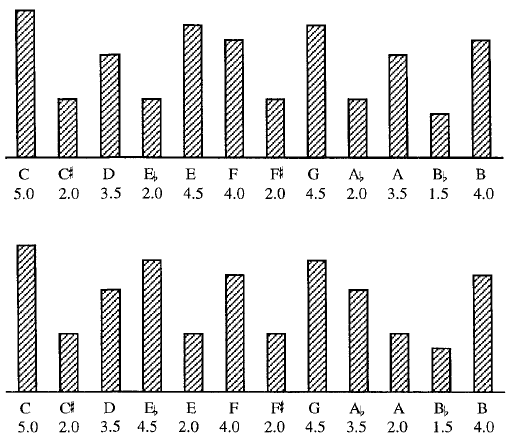
\includegraphics[scale=0.6]{CBMS/temperley_mod_keyprofile.png}
	\end{center}
	\legend{Fonte: \cite[pg. 174]{temperley2001cognition} }
\end{figure}



\pagebreak
\section{Restrições Cognitivas versus Segmentação Atonal}


Quase 10 anos após a publicação da GTTM Lerdahl publica um ensaio chamado \textbf{"Restrições cognitivas nos sistemas composicionais"}\cite{lerdahl1992cognitive}, ancorando observações em uma aproximação bastante conservadora e crítica da música serial, tomando como caso a peça "Le Marteau Sans Maitre" de Pierre Boulez, e defendendo a tese de que uma música tão distante dos perfis cognitivos básicos da musica tonal seria inapreensível para os sentidos\footnote{Conferir também o ensaio de Milton \citeonline{babbitt1958cares} chamado "Who Cares If you Listen" que argumenta o inverso: pressupostos que sustentariam uma pesquisa \textbf{despreocupada da escuta leiga} e que necessita o suporte da ciência para abrir novas fronteiras no desconhecido, assim como ocorre com as ciências exatas não-aplicadas. }. 

É importante levar em conta que a GTTM e suas derivações insistiram sempre numa afirmação de uma suposta preferência cognitiva regida pelos princípios "atrativos" tonais, o que pode ser interessante em teorias pós-tonais para pensar ambiguidade de sistemas que induzem uma intenção auditiva politonal, \textbf{mas não parece ser suficiente }para pensar critérios que considerem uma busca auditiva pelas sonoridades de grupos de intervalos não organizados a partir da suposta ordem dos "espaços de alturas tonais"\cite{lerdahl1988tps} intuídos pela cognição de uma escuta ocidentalizada ou ocidentalizante.

Cabe pensar aqui aquilo que \citeonline[pg.18-20]{nattiez2001tripartite} diferencia como estésica externa e estésica indutiva. 

\textbf{Estésica externa} é aquela baseada em critérios que entrariam na análise por via de uma comprovação de pesquisa de campo, buscando legitimar que os paradigmas apontados são estatisticamente comuns para a percepção de um determinado grupo de ouvintes. 

Já a \textbf{estésica indutiva} seria determinada por uma inferência explícita e autoral do musicólogo, que aponta aquilo que segundo seus próprios critérios poderia ser percebido como relevante e importante numa escuta. 

Mas seria possível trabalhar um interesse \textbf{apenas estrutural} no material, isolado de seu contexto de condicionamento da escuta ou intenção do compositor? Nattiez chama de \textbf{"nível neutro"}, \textbf{"análise imanente"} ou \textbf{"análise material"} as estruturas em estado bruto. Dados quantitativos ainda isoladas de seu contexto argumentativo. 

A teoria de grupos e classes de alturas sempre foi evitada pela linha descendente da pesquisa da GTTM, justamente por não parecer tão preocupada em afirmar seus pressupostos em pesquisas de campo sobre cognição. Por estar preocupada apenas com o \textbf{"nível neutro"} quando a aplicada em análises sempre acabaria induzindo seus apontamentos em critérios subjetivamente determinados pelo musicólogo. Por outro lado a normatização que as teorias derivadas da GTTM impõe parecem tender a uma limitação estanque. Por que limitar a percepção naquilo que supostamente seria a percepção do ouvinte médio? Não seria produtivo propor outros modos de escuta, mesmo que ainda não estejam condicionados?

Em seu artigo sobre critérios para uma análise da música atonal \citeonline{lerdahl1989atonal} afirma:

\begin{citacao}
Como a descrição teórica da classe de alturas e conteúdo da classe de intervalos relaciona-se com a organização das alturas na superfície musical? A relação frequentemente parece remota. As noções de "classe de altura" e "classe de intervalo" são abstrações da altura e intervalo de uma passagem musical. E os vários conceitos invocados para equivalência entre grupos ou similaridade (equivalência por inversão, forma normal, vetores de intervalo, relação Z, relação R, relação de inclusão, complexos K e Kh) também criam um distanciamento da superfície. Não há nada errado com este princípio: todas as teorias generalizam desde o fenômeno. A questão é se realmente estas abstrações em particular refletem e iluminam nossa escuta. A pouca pesquisa de campo feita nestes assuntos (...) não tem sido muito encorajadora."\cite{lerdahl1989atonal}
\footnote{
How does the theoretical description of pitch-class and interval-class content relate to the listener's organization of pitches at the musical surface? The relationship often seems
remote. The very notions "pitch class" and "interval class" are abstractions from
the pitch and interval content of a musical passage. And the various concepts
invoked for set equivalence or similarity (inversional equivalence, normal form,
interval vectors, Z-relatedness, the R relations, the inclusion relation, the K and
Kh complexes) also create a distancing from the surface. There is nothing wrong
with this in principle: all theories generalize from phenomena. The question is
whether these particular abstractions reflect and illuminate our hearing. The little
experimental research that has been done on such matters (...) has not been very encouraging.
\cite{lerdahl1989atonal}}
\end{citacao}

Consideramos esta negação arbitrária e suspeita. Se as teorias de classes de alturas são tão distantes da realidade da escuta por que continuam sendo cada vez mais formalizadas? Nos pareceu essencial um estudo comparado da abordagem cognitivista com este este contraponto das teorias de classes da altura, justamente por estas partirem de outros pressupostos. Faremos um percurso por estas teorias no próximo capítulo.


\chapter{Teorias de Grupos das Classes de Alturas para uma Segmentação Atonal }
\label{modelos}

Vimos na teoria do "solfejo das classes de altura"\cite[p. 115]{temperley2001cognition} de David \citeonline{temperley2001cognition} a categorização de uma divisão de grupos de altura que ele denomina "Altura de Classes Tonais"\cite[p. 115]{temperley2001cognition}. Neste capítulo exploramos teorias pós-tonais que são geralmente evitadas pela abordagem cognitivista por partirem de princípios de agrupamento que não são argumentados por uma funcionalidade tonal normativa, mas sim pela formalização de relações de simetria, similaridade e transformação entre os doze intervalos cromáticos que trariam o sentido musical por outros tipos de fruição da forma musical. 

Na teoria de grupos de classes de altura ("Pitch Class Theory") os intervalos são tratados de maneira neutra em relação a qualquer centro tonal pré-determinado e parte-se do princípio de que agrupamentos de alturas podem gerar estruturas de derivadas por uma espécie de parentesco intervalar, incluindo a similaridade por inversão ou retrógrado destes como veremos mais adiante. 

Estas teorias são fortemente influenciadas pela ideia de serialismo formalizada pelo dodecafonismo frequentemente atribuído a Arnold Shoenberg e seus pupilos da segunda escola de Vienna, mas é bom lembrar que o pensamento serial é um pensamento composicional que pode também ser encontrado em compositores muito anteriores a estas formalizações, portanto podemos encontrar esta abordagem analítica sendo usada para destacar aspectos de composições de outros contextos que não o restrito ao repertório atonal clássico, como faz por exemplo Joel \citeonline{lester1989analytic} em sua didática para análises de um repertório pós-tonal do ínicio do século XX ou Allen Forte na sua tese sobre a "Sagração da Primavera" de Stravinski\cite{forte1978harmonic}.

\begin{citacao}
Foi, obviamente, Allen Forte quem foi o pioneiro das análises com a taxonomia dos grupos de classes de alturas aplicadas em conceitos da matemática, primeiro surgindo em tipos de Milton Babbit (a teoria conceitual), e em seguida com a inclusão e abstração de relações (como as relações de similaridade) construídas para uso analítico. A "teoria de grupos" de Forte (...) tem tido suas próprias ramificações e influência. Em particular, as próprias análises de Forte de peças individuais tem levado muitos outros a fazerem de maneira parecida, e a ideia inicial de Forte das relações de similaridade ( diferentes das relações de equivalência) sobre os grupos de classes de alturas tem visto florescer uma indústria teórica em torno disto, depois que os artigos seminais de Morris, Rahn  Lewin apareceram em 1980.\cite{rahn2004swerve}\footnote{
It was, of course, Allen Forte who in the USA pioneered the analytical with a taxonomy of pc-set application of concepts from mathematics, first arose also in serial Babbittian types (the concept theory), and following as some inclusion and with relations abstract up (such similarity relations) meant for analytical use. Forte's "set theory" (...) has had its own ramifications and influence. In particular, Forte's own analyses of individual pieces of music have led many others to do likewise, and Forte's initial idea of similarity relations (as distinct from equivalence relations) among pitch-class sets has seen a flourishing theoretical industry grow around it, after seminal articles by Morris, Rahn, and Lewin appeared in 1980.\cite{rahn2004swerve}}
\end{citacao}




Com formalização de uma teoria de grupos de classes de alturas pela geração de musicólogos e compositores seriais da segunda metade do século XX e com os avanços exponenciais da computação nas últimas décadas estas teorias vão sendo testadas e aplicadas a ponto de já constituírem uma área bastante específica da musicologia contemporânea.\cite{aroundset2013}

Um exemplo de interesse do presente trabalho é a classe de objetos "Math Tools"\cite{andreatta2003implementing,AndreataOMtutorial,DebrilOM} da linguagem de programação OpenMusic\footnote{ver \autoref{OMmath}}, que organiza em orientação a objetos muitos dos conceitos que veremos logo a seguir. 



\section{Fórmulas de agrupamento e transformação dos intervalos}

A teoria de grupos de classes de altura utiliza como base de suas formulações a relação entre os 12 semitons da escala cromática de forma modular: considerando alturas de mesma oitava como sujeitas a mesmas propriedades intervalares, podendo argumentar relações independentes de registro. Exemplo: O Dó grave representado no protocolo MIDI pelo valor 24 tem uma relação de equivalência com o Dó agudo de valor 72. A fórmula é simples: ambos quando divididos por 12 apresentam resto 0. A nota Ré, por exemplo, sempre apresentaria o resto 2, e assim por diante. Dizemos por tanto que pertencem a uma mesma classe de altura.

Diferente de quando argumentada uma enarmonia funcional\footnote{ver \autoref{solfejo} } (como por exemplo D\# $\to$ Eb ) a teoria de grupos e classes de altura não toma como princípio ideias do tipo "terça maior ou menor", "nota sensível" ou "nota de passagem" pois vai partir de uma relação direta entre os aglomerados sonoros, buscando similaridades e equivalências sem estar tão presa as formas de prolongamento normatizadas pelo tonalismo clássico.\cite{lerdahl1989atonal,straus1987problem}

Os intervalos são antes de funções, distâncias. Nas teorias de classes de alturas estas distâncias podem estar categorizadas como intervalos ordenados - usando número negativos para os intervalos descendentes, ou não-ordenados - considerando intervalos equivalentes independentes de suas direções.\cite[pg. 6]{straus2004}

Isso cria imediatamente uma relação interessante de parentesco entre pares em todos intervalos da escala cromática exceto para os trítonos, intervalos de sexta ordem, que está equidistante de 0 e 12 e portanto não possui uma inversão propriamente dita, mas sim tem o papel de cortar ao meio este espelhamento.

\begin{figure}[!h]
	\caption{\label{fig_grafico}Equivalência de intervalos por inversão }
	\begin{center}
	    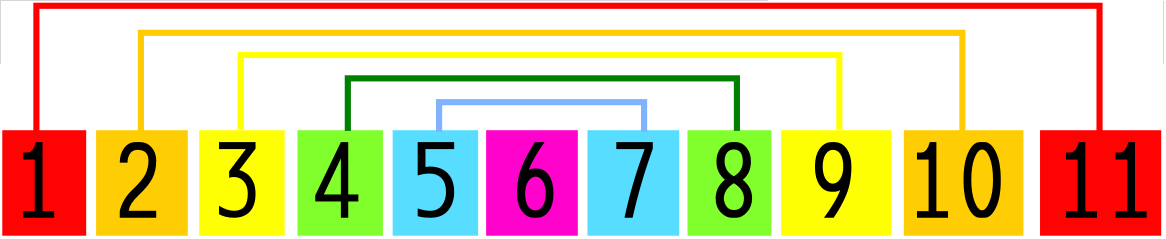
\includegraphics[scale=0.3]{algo/equivalencia_inversa.png}
	\end{center}
	\legend{Fonte: autor }
\end{figure}




\subsection{Vetor intervalar}

A operação obtenção do vetor intervalar é a primeira das reduções sugeridas para propor uma similaridade entre agrupamentos que seja neutra quanto inversões e oitavas.

Tomemos um exemplo de um cluster C-D-E-Bb.



\begin{figure}[!h]
	\caption{\label{fig_grafico}[0,2,4,10] }
	\begin{center}
	    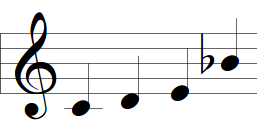
\includegraphics[scale=0.6]{OM_settheory/vetor02410.png}
	\end{center}
	\legend{Fonte: autor }
\end{figure}


Este trecho pode ser reduzido a sequencia de alturas [0,2,4,10]

Organizamos seus intervalos fazendo todas as combinações possíveis entre estas distâncias:


$ inversões = \left\{
  \begin{array}{l l}
    2-0 = 2\\
    4-0 = 4\\
    10-0 = 10 \\
     \\
    4-2 = 2\\
    10-2= 8 \\
     \\
    10-4= 6
  \end{array} \right.
$

O vetor de intervalos pode ser reduzido então a uma contagem que coloca no mesmo grupo os intervalos que são inversões dos primeiros 5 intervalos possíveis, já que seus pares apos o trítono no são considerados espelhamentos. No exemplo acima temos 10 que é a inversão de 2 e 8 que é a inversão de 4. Portanto nosso vetor fica assim:


\begin{table}[h]
\begin{tabular}{|
>{\columncolor[HTML]{FD6864}}l |
>{\columncolor[HTML]{F8A102}}l |
>{\columncolor[HTML]{F8FF00}}l |
>{\columncolor[HTML]{34FF34}}l |
>{\columncolor[HTML]{00D2CB}}l |
>{\columncolor[HTML]{EE00EE}}l |}
\hline
1 & 2 & 3 & 4 & 5 & 6 \\ \hline
0 & 3 & 0 & 2 & 0 & 1 \\ \hline
\end{tabular}
\end{table}

Pode-se dizer então que a classe de alturas [0,2,4,10] possui o vetor intervalar <0,3,0,2,0,1>.


\subsection{Forma Normal} 

É comum na prática de uso dos grupos de classes de altura a preparação dos conjuntos em sua forma ordenada e reduzida. Desta maneira podemos mais facilmente reconhecer as equivalências entre os grupos, reconhecer transposições, propriedades.


\begin{figure}[h]
	\caption{\label{fig_grafico}Redução de um segmento do Microkosmos 101 de Bártok para um cluster de 4 alturas. }
	\begin{center}
	    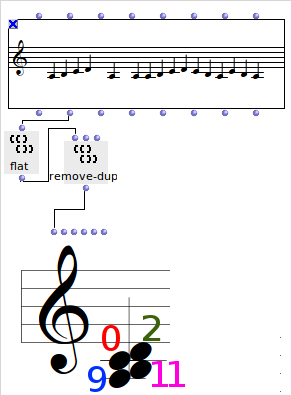
\includegraphics[scale=0.7]{OM_settheory/reducao_acorde.png}
	\end{center}
	\legend{Fonte: autor }
\end{figure}

Para a redução de uma forma normal partimos do cluster sem repetições, colocando todas as alturas dentro da mesma oitava. Os passos seguintes são: 
\textbf{a)} Ordenar de forma ascendente e escolher a sequencia que tenha a menor distância da primeira até a última nota.
\textbf{b)} Se houver empate reduzir pela que seja mais compacta à esquerda comparando o menor intervalo entre a primeira e penúltima e assim por diante.s
\textbf{c)} Havendo ainda empate, escolher aquele grupo que tem a menor altura como início. 

\begin{figure}[h]
	\caption{\label{fig_grafico}Forma Normal. }
	\begin{center}
	    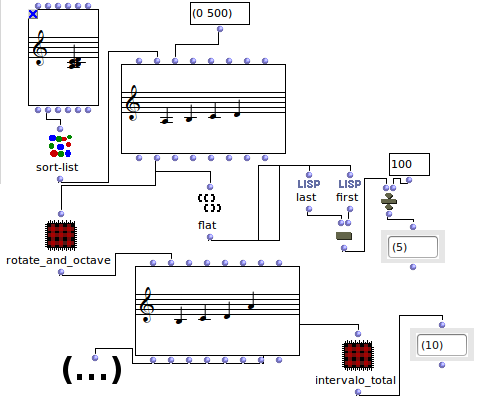
\includegraphics[scale=0.7]{OM_settheory/forma_normal.png}
	\end{center}
	\legend{Fonte: autor }
\end{figure}



\pagebreak
\subsection{Forma Prima} 

A forma prima é um procedimento para simplificar ainda mais a forma normal, encontrando "a mais normal das normais"\cite[p.47]{straus2004} e reduzindo vetores que possuem os mesmos intervalos ou são inversões e transposições a um vetor primário. Para isso uma forma normal é transposta até que possua o zero em sua primeira posição. Assim é feito também com sua inversão. A forma mais compacta à esquerda será a forma prima. Allen \citeonline{forte1973structure} desenvolveu uma taxonomia a partir das formas primas que tem sido utilizada como forma canônica para representação de grupos de classes de altura.\footnote{A biblioteca "math" do OpenMusic possui o objeto "p-form" para encontrar os agrupamentos de Forte. A tabela original está no livro "The Structure of Atonal Music"\cite[p.179-181]{forte1973structure}}. Forte organiza agrupamentos pelo número de elementos seguidos por um número que diz qual ordem dentro do conjunto com aquele mesmo número de elementos. Exemplo: |3-1| é composto das alturas (0,1,2), |3-2|  é o cluster (0,1,3), |4-17|  é composto por (0,3,4,7), e assim por diante.

\begin{figure}[h]
	\caption{\label{fig_grafico}Fórmulas de agrupamento de classes de altura. }
	\begin{center}
	    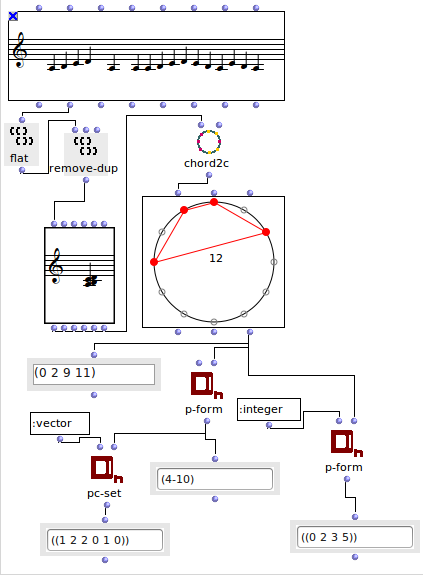
\includegraphics[scale=0.7]{OM_settheory/forma_prima_forte_vector.png}
	\end{center}
	\legend{Fonte: autor }
\end{figure}





%\begin{citacao}
%Two Algorithms for Computing the Prime Form

%There are two algorithms for computing the prime form of a Pitch Class Set. The first was introduced by Allen Forte %in The Structure of Atonal Music and the second is used by John Rahn in his book Basic Atonal Theory and is also %used by Joseph N. Straus in his Introduction to Post-Tonal Theory.

%The difference between the two algorithms is apparent when examining Pitch Class Set 6-31. The Prime Form using the %Forte algorithm is (0,1,3,5,8,9), and the prime form using the Rahn algorithm is (0,1,4,5,7,9). As you can see, the %Forte algorithm puts a priority on making the small numbers smaller (i.e. 3 instead of 4), whereas the Rahn %algorithm wants the larger numbers to be smaller (i.e. 7 instead of 8).

%Which is better? Well, it depends on who you ask. Computer programmers and computer music people will typically %prefer the Rahn algorithm because it is computationally more elegant. However, the Forte algorithm has the more %established pedigree, and so it tends to be preferred by academics.

%Fortunately, this is usually a minor issue because it only affects the following 5 sets:

%Pitch Class Set	Forte Prime	Rahn Prime
%5-20	(0,1,3,7,8)	(0,1,5,6,8)
%6-Z29	(0,1,3,6,8,9)	(0,2,3,6,7,9)
%6-31	(0,1,3,5,8,9)	(0,1,4,5,7,9)
%7-20	(0,1,2,4,7,8,9)	(0,1,2,5,6,7,9)
%8-26	(0,1,2,4,5,7,9,10)	(0,1,3,4,5,7,8,10)
%\end{citacao}


\subsection{Singularidades nos agrupamentos }

Algumas propriedades entre os grupos de classes de alturas são muito interessantes como princípio composicional, e mesmo quando não tao obvias em primeiras audições, ao menos ajudam garantir alguma coerência estrutural conceitual. George Perle argumenta sobre "funções motívicas" em grupos de de alturas\cite[ p.60-85]{perle1991serial} e observa algumas estratégias de compositores para aproveitar algumas propriedades encontradas em relações internas das series. Perle no entanto mostra-se cético a formalização de nomenclaturas analíticas derivadas da classificação de Allen Forte e sua aplicação em argumentações para análises de composições que tenham sido compostas antes fórmulas tornarem-se ferramentas musicológicas.\cite{perle1990pitch}

Levantaremos aqui algumas destas propriedades conforme o resumo didático proposto por \cite{straus2004}, sem ainda estarmos certos de sua efetividade para analises mas interessados na formalização computacional possível destas para processos composicionais.


\subsubsection{Notas Comuns sob transposição}

Tomemos o seguinte exemplo: Dado um grupo em sua forma prima [0,2,5] - ou "4-10" na forma prima pela classificação de Allen \citeonline{forte1973structure} - quando transpomos para o intervalo 2 e seu inverso 10, obtemos duas notas iguais para cada um destes grupos.

\begin{figure}[!h]
	\caption{\label{fig_grafico}Notas comuns na transposição. }
	\begin{center}
	    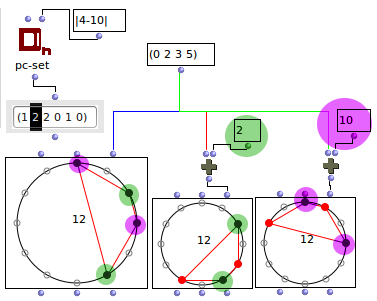
\includegraphics[scale=0.7]{OM_settheory/notas_comuns_2e10.png}
	\end{center}
	\legend{Fonte: autor }
\end{figure}



Isso acontece porque o vetor de intervalos para esta forma é <1,2,2,0,1,0> e podemos observar que há uma fórmula geral que prova que o número de incidências comuns de uma determinada classe de alturas em sua transposição será o número de repetições deste intervalo em seu vetor original. Neste caso por exemplo temos duas incidências do intervalo de classe 2 portanto as transposições T2 e T10 terão duas notas em comum com T0.

Há uma exceção a esta regra:
 
\begin{figure}[!h]
	\caption{\label{fig_grafico}Notas comuns na transposição com trítono. }
	\begin{center}
	    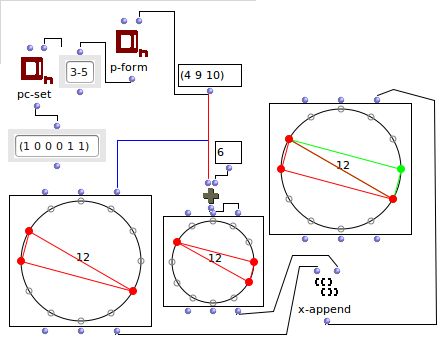
\includegraphics[scale=0.7]{OM_settheory/notas_comuns_tritono.png}
	\end{center}
	\legend{Fonte: autor }
\end{figure}

É preciso observar que para o caso do trítono a inversão é simétrica, portanto para cada trítono teremos duas notas em comum. Como no exemplo acima: 10 e 4 geram as duas simétricas 4 e 10 e portanto um trítono gerou duas notas em comum e assim por diante.

Interessante pensar também que o vetor de intervalos irá determinar transposições onde não existem notas nenhumas em comum. Composicionalmente isso pode ser visto como uma possibilidade de transpor para uma sessão totalmente distinta da anterior, criando algum discurso com estas transições.


\subsubsection{Simetria Transpositiva}

Na simetria transpositiva temos um padrão de intervalos que funciona como palíndromo (tem a mesma leitura da esquerda para a direita e direita para esquerda).

\begin{figure}[!h]
	\caption{\label{fig_grafico}A simetria transpositiva é obtida através de um padrão de intervalos palíndromo. }
	\begin{center}
	    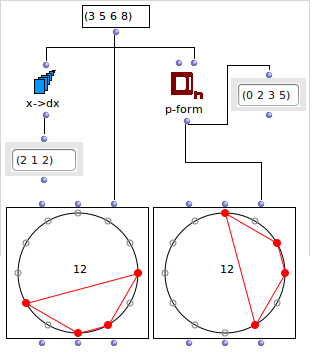
\includegraphics[scale=0.6]{OM_settheory/palindrome1.png}
	\end{center}
	\legend{Fonte: autor }
\end{figure}



\begin{figure}[!h]
	\caption{\label{fig_grafico}A forma circular é mais geral do que a numérica para a visualização do padrão de simetrias. }
	\begin{center}
	    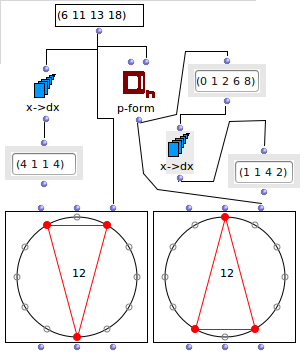
\includegraphics[scale=0.6]{OM_settheory/palindrome2.png}
	\end{center}
	\legend{Fonte: autor }
\end{figure}



\subsubsection{Complemento}

Útil para reconhecer e produzir contextos totalmente distintos entre si, o complemento é composto por todos intervalos que estão exclusos dos grupo, produzindo um outro grupo completamente diferente.


\begin{figure}[!h]
	\caption{\label{fig_grafico}O complemento contém todas alturas cromáticas que o conjunto original não possui. }
	\begin{center}
	    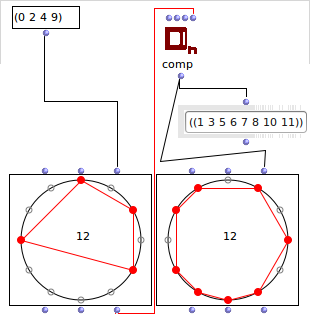
\includegraphics[scale=0.6]{OM_settheory/complemento.png}
	\end{center}
	\legend{Fonte: autor }
\end{figure}


\subsubsection{Relação Z entre grupos de classes de alturas}

A relação Z é uma das interessantes relações onde há uma equivalência sem que os conjuntos sejam transposições ou inversões entre si, neste caso produzindo dois conjuntos que possui os mesmos intervalos na sua constituição.


\begin{figure}[!h]
	\caption{\label{fig_grafico}Dois conjuntos Z-relacionados possuem os mesmos intervalos sem serem inversões ou transposições um dos outros. }
	\begin{center}
	    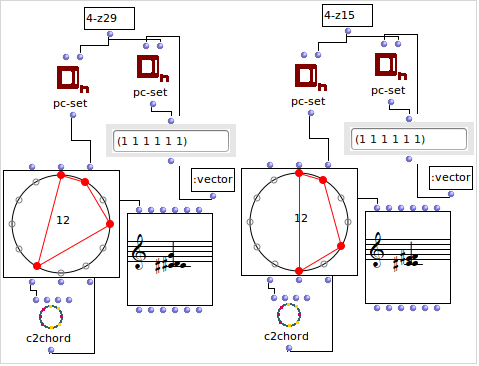
\includegraphics[scale=0.7]{OM_settheory/Z_related.png}
	\end{center}
	\legend{Fonte: autor (adaptado de exemplo do tutorial MathTools do OM) }
\end{figure}


George Perle exemplifica a relação Z como uma das relações que não são intuitivas em sua rotina composicional:

\begin{citacao}
Mas nenhum destes argumentos teria qualquer peso para mim se eu pudesse ao menos escutar as correspondências que Forte descreve. Eu posso descobrir estas conexões entre coleções Z-relacionadas somente sujeitando-as a um escrutínio analítico que não tem nada a ver com minha experiência intuitiva como ouvinte ou compositor. Ou, para falar de maneira mais sincera, permitir que o Professor Forte conduza seu escrutínio analítico para mim.
\cite[p.168]{perle1990pitch}\footnote{
But none of these arguments would carry any weight with me if
I could only hear thes correspondences that Forte describes. I can
discover these connections between Z-related collections only by sub-
jecting them to an analytical scrutiny that has nothing whatever to do
with my intuitive experience as a listener or as a composer. Or, to
speak more candidly, by allowing Professor Forte to conduct this
analytical scrutiny for me. 
\cite[p.168]{perle1990pitch}}
\end{citacao}

Perguntamo-nos se este tipo de afirmação não seria um tanto arbitrária, afinal as diferenças entre terças maiores e menores não são também no fundo resultado de uma exposição cultural associativa a esta nomenclatura e consequentemente a sua geometria e particularidade numérica em relação a uma funcionalidade dentro dos grupos diatônicos a quais pertencem? Se tudo entao e um condicionamento cultural da escuta por onde buscar novas escutas?

Parece que de alguma maneira a relação Z acaba por nomear uma sonoridade por uma particularidade entre relação numérica e geométrica curiosa, e no mínimo serve como mnemônico de uma relação entre estas sonoridades.

\subsection{Arbitrariedade e indução  na segmentação atonal}

Encontrar estas relações em composições anteriores a sua formalização é que obviamente é um problema para uma estésica indutiva\cite{nattiez2001tripartite} que se vale de todos esforços documentais para provar o quanto esta atitude composicional já existiu inconscientemente em gestos instrumentais não condicionados pela geometria constatada.


Esta questão sobre arbitrariedade na busca por estas particularidades de relações entre grupos em análises de peças principalmente anteriores a estas formulações nos parecem no fundo uma aporia. Esforços foram feitos de todas as maneiras para comprovar a tanto a eficacia quanto a ineficácia do sistema para aplicação em analises, como por exemplo a tese de Ethan \citeonline{haimo1996atonality} buscando "falácias" no esquema analítico clássico de teoria de grupos quando confrontado com anotações originais de Arnold Shoenberg.

\citeonline{straus2004} sentencia:

\begin{citacao}
A resposta é que você não pode saber com antecedência.
Você tem que entrar no mundo da peça – ouvindo, tocando, e cantando – até que você
obtenha um senso de quais ideias musicais são fundamentais e recorrentes. No processo,
você encontrar-se-á movendo-se em torno de um tipo familiar de círculo conceitual. Você
não pode saber quais são as principais ideias até que você as veja recorrer; mas você não
pode encontrar recorrências até que você saiba quais são as ideias principais. A única
solução prática é bisbilhotar a peça, propondo e testando hipóteses conforme você
prossegue. 
\cite{straus2004}
\end{citacao}

\citeonline{nattiez2003allen} faz uma crítica minuciosa da aplicação da teoria de grupos das classes de altura derivada do trabalho de Allen Forte, em busca de uma descrição estésica que justifique a aplicação de toda a formalização de seu nível neutro de nomenclaturas e chega a seguinte conclusão:


\begin{citacao}
(...)seria fascinante ver que resultados obteríamos comparando grupos quais descreveriam unidades previamente segmentadas por uma análise paradigmática num nível neutro. Se nos sentimos intimidados a confiar nas análises preliminares, com efeito, o caleidoscópio com qual o analista vai descobrir trabalhos atonais vai efetivamente ser fruto de operações mágicas, não porque o compositor escondeu-as ali, mas porque o musicologista, através do truque com as mãos, esta agindo como um mágico!\cite[ p.16]{nattiez2003allen}\footnote{(...)it would be fascinating to see what results we would obtain from comparing sets which would describe units previously segmented by a paradigmatic analysis at the neutral level. If we do feel compelled to rely on this preliminary analysis, in effect, the kaleidoscope which the analyst will discover in atonal works will effectively be the fruit of magical operations, not because the composer hid them there, but because the musicologist, through sleight of hand, was acting like a magician!
\cite[ p.16]{nattiez2003allen}}
\end{citacao}






% ----------------------------------------------------------
% PARTE
% ----------------------------------------------------------
\part{Implementação Computacional}
\label{computacional}
% ----------------------------------------------------------


\chapter{Composição Assistida por Computador}

O objeto de estudo desta pesquisa são os algoritmos de manipulação de dados de uma superfície musical normatizada para a escala de temperamento igual, de doze tons ou "12-TET"\cite[ p.76]{sethares2005tuning}, tradicionalmente usada nas partituras da prática comum. Estamos abstraindo no momento as questões como timbre, microtonalismo, afinações ou qualquer outros aspectos não formalizáveis em partitura tradicional. 

Curiosamente, a chamada "computer music"\cite{curtis1996computer} que derivou dos primeiros mainframes e seus métodos estocásticos de compositores como Hiller e Xenakis, parece cada vez mais seduzir para um estudo da música que inicia pela morfologia do espectro sonoro, onde impera o "microsom"\cite{roads2004microsound} manipulado nos níveis limite da psicoacústica. Interessa em nossa abordagem repensar um pouco os limites desta manipulação simbólica de escalas e aglomerados de alturas, antes de mergulhar nas possibilidades expandidas. 

O criador da linguagem PureData, categoriza esta diferença no prefacio do "Open Music Composer's Book 1"\cite{OM_book01_2006}:

\begin{citacao}
O campo da computer music pode ser pensado como tendo dois ramos fundamentais, um preocupado com a manipulação de sons musicais, e outra preocupada com a com a representação simbólica da música. (...) Os dois ramos podem provisoriamente serem chamados pelos nomes "Musica Gerada Por Computador" (o termo de Denis Baggi) e "Composição assistida por computador" - ou pelos acrônimos MGC e CAC."\cite[pg. ix]{puckettecomputing}\footnote{
The field of computer music can be thought of as having two fundamental branches, one concerned with the manipulation of musical sounds, and the other concerned with symbolic representations of music. (...) The two branches might provisionally be given the names “Computer Generated Music” (Denis Baggi’s term for it) and “Computer Aided Composition”— or CGM and CAC for short.\cite[pg. ix]{puckettecomputing}}

\end{citacao}




\section{Linguagens Dataflow}
\label{ferramentas}

As linguagens de programação PureData e OpenMusic tem ao menos duas coisas em comum: ambas utilizam o paradigma de programação dataflow – uma representação gráfica dos algoritmos que deixa os programas similares a caixas conectadas por cabos, estimulando a imaginação para algo mais tátil do que cálculos abstratos.

Ambas também são linguagens surgidas a partir de projetos surgidos no IRCAM (Institut de Recherche et Coordination Acoustique/Musique) a instituição francesa que tem entre seus idealizadores o compositor Pierre Boulez e é pioneira em pesquisas computacionais guiadas por processos composicionais. São descendentes diretas da primeira geração de linguagens musicais dataflow: Patchwork (OM) e Max (PD).

Considerando que são ainda muito utilizadas por pesquisadores de Composição Assistida por Computador (CAC) e Música Algorítmica, estas já podem já de alguma forma serem consideradas linguagens de computação musical com relevância histórica o suficiente para no mínimo servirem de base para novas invenções.

Utilizamos nesta pesquisa ambas as linguagens testando suas limitações e disponibilidade de bibliotecas já prontas e bem documentadas. 



\subsection{OM}

\begin{citacao}
"Enquanto a maioria das “linguagens de programação musical” lidam principalmente com processamento de sinal e síntese
sonora, uma abordagem original adotada pelo time de representação musical do IRCAM no fim dos anos 80 foi
particularmente um foco na nas estruturas simbólicas e processos musicais, isto é, aspectos tradicionalmente
ignorados ou deixados de lado dos ambientes computacionais."\cite{bresson2011openmusic}
\end{citacao}

Em suma, o OpenMusic teve ( pelo menos em seus primeiros anos ) uma intenção mais voltada para processos preocupados com a continuidade dos sistemas derivados dos estudos eruditos de intervalos, acordes, harmonia que estavam na base das preocupações do serialismo integral. O OM sempre foi um dos software amplamente utilizados para tal fim, e isto reflete diretamente em sua interface e cultura de uso.

O OM é um framework que tende a uma programação orientada pela reflexão em tempo diferido, isto é, estimula a composição por escolha entre diversos resultados permutados e decupados em um tempo de escuta.

Organiza materiais basicamente orientado pela escrita e fortemente pensado dentro do esquema de intervalos melódicos
harmônicos derivados da notação moderna para música orquestral, utilizando sequenciadores bastante similares ao pentagrama de pauta sem ( “chord-seq”) ou com figuras de compasso (com o sequeciador “voice” ).

\subsubsection{chord-seq}

A linguagem OpenMusic tem objetos avançados para a manipulação e sequenciamento de estruturas em representação partitural. Desde objetos gráficos para representação da nota em pauta, acordes isolados ou mesmo estruturas em árvore para construção de ritmos compostos ("mktree") e polifonia ("voice"). Estes objetos podem ser organizados em macro estruturas de sequenciamento, como as "maquettes" e "sheets"\cite{bresson2008scores}.

Importante destacar aqui o funcionamento do objeto \textbf{"chord-seq"}  para o detalhamento de como opera a lógica dos encadeamentos de acordes, que por trás dos objetos gráficos são entendidos como listas Lisp\footnote{ Para detalhes sobre a linguagem de programação LISP, c.f. \cite{graham1995ansi}} aninhadas, utilizando uma escala de "midicents" onde entre cada semitom da escala cromática e possível também uma divisão de 100 microtons. (por exemplo: ao invés de representar um Dó com o número 12, 24, 48, etc. será reresentado por 1200, 2400, 4800,etc.). Na figura abaixo detalhamos o funcionamento das entradas e saídas de um objeto "chord-seq".

\begin{figure}[!h]
	\caption{\label{fig_grafico}Objeto Chord-Seq do Opem Music}
	\begin{center}
	    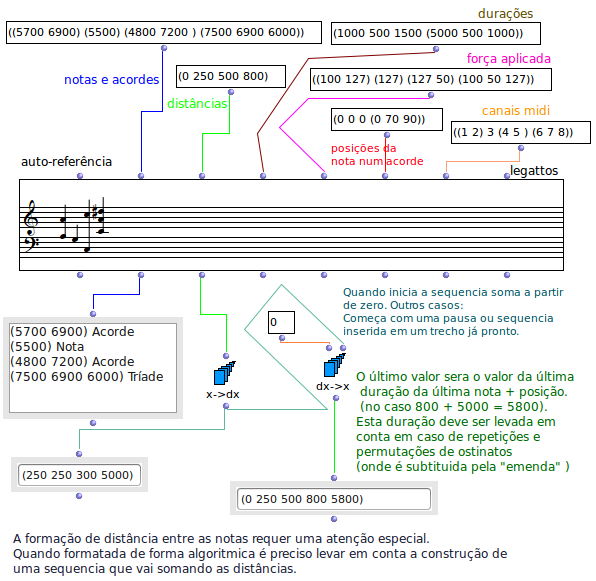
\includegraphics[scale=0.7]{OMPD/chord-seq-sem-titulo.png}
	\end{center}
	\legend{Fonte: autor }
\end{figure}



\subsubsection{Listas de dados}

O OM implementa uma série de operações sobre as listas de dados estruturadas. Abaixo selecionamos algumas funções básicas que auxiliam na manipulação dos dados dentro do OM.

\begin{figure}[!h]
	\caption{\label{fig_grafico}Operações com listas no OMs}
	\begin{center}
	    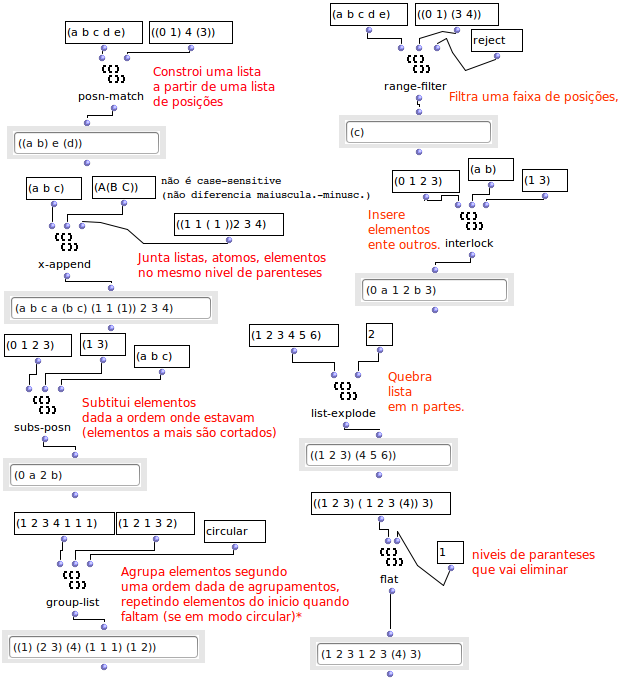
\includegraphics[scale=0.7]{OMPD/OM-listas01.png}
	\end{center}
	\legend{Fonte: autor }
\end{figure}

\begin{figure}[!h]
	\caption{\label{fig_grafico}Operações com listas no OMs}
	\begin{center}
	    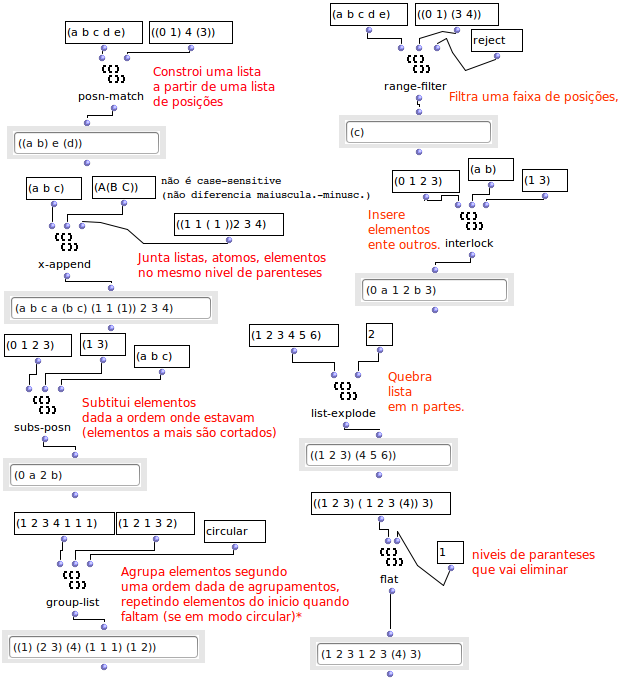
\includegraphics[scale=0.7]{OMPD/OM-listas01.png}
	\end{center}
	\legend{Fonte: autor }
\end{figure}


\subsubsection{Operações combinatórias e operações sobre grupos de classes de altura }
\label{OMmath}
O OM possui também algumas classes já preparadas especialmente para organizar series, permutar, ordenar, embaralhar e inclusive uma classe chamada "math", que antecipa e organiza uma serie de operações básicas sobre grupos de classes de altura, como extração do vetor intervalar, classificação de conjuntos de Allen Forte e uma representação gráfica da geometria das classes de altura, o objeto "n-cerle"\cite{andreatta2003implementing}. Alguns objetos desta classe foram testados nas demonstrações do \autoref{modelos}.

\begin{figure}[!h]
	\caption{\label{fig_grafico}Alguns objetos para operações combinatórias e operações em grupos de classes de altura no OMs}
	\begin{center}
	    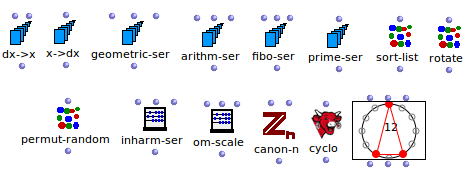
\includegraphics[scale=0.7]{OMPD/series-OM.png}
	\end{center}
	\legend{Fonte: autor }
\end{figure}

O OM também incorpora dentro de seus sequenciadores de nota um procedimento para segmentar articulações com fins de análise, preparando-os para uma classificação de grupos de alturas com a estrutura de dados do objeto "n-cercle"\cite{bresson2012new}.

\begin{figure}[!h]
	\caption{\label{fig_grafico}Segmentação em Chord-Seq de OpenMusic}
	\begin{center}
	    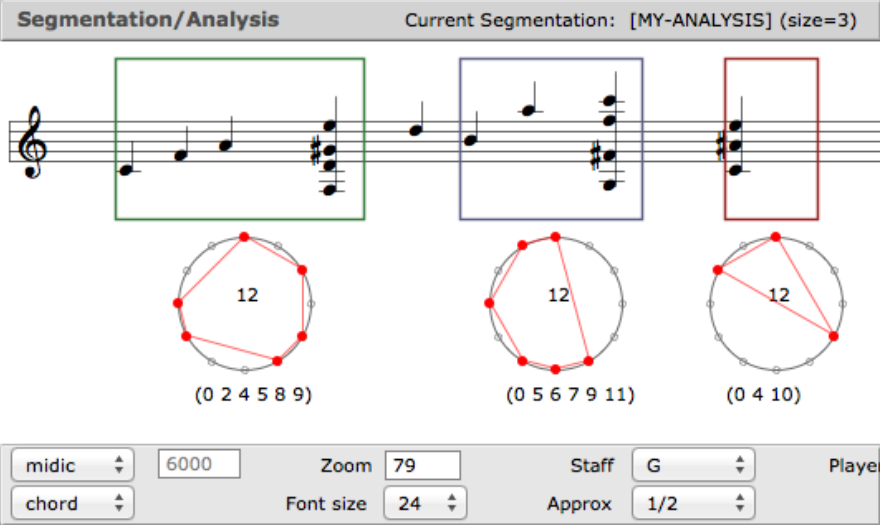
\includegraphics[scale=0.4]{OMPD/segmentaOM.png}
	\end{center}
	\legend{Fonte: \cite{bresson2012new} }
\end{figure}


\pagebreak
\subsection{PD}

Desde o início de seu desenvolvimento o PureData surge como um software preocupado em resolver problemas de processamento digital de sinal de maneira estruturada, paralelo ao momento que sua versão comercial Max\footnote{\url{http://cycling74.com/} Acesso em 10 de julho de 2014.} desenvolvia sua versão "MSP" para processamento de áudio digital, baseada neste primeiro estágio do PD. 

\begin{citacao}
Um novo sistema de software, chamado Puredata, está em seus primeiros estágios de desenvolvimento. Seu design almeja remediar algumas deficiências do programa Max e preservar algumas de suas vantagens. A mais importante fraqueza do Max é a dificuldade de manter estruturas de dados compostas de um tipo que possa ser acessado quando analisando e ressintetizando sons  ou quando gravando e modificando sequencias de diferentes tipos. Também, tem sido difícil integrar sinais que não sejam de áudio (vídeo por exemplo, e também espectro sonoro ) dentro do rígido sistema de “objetos til” ($\sim$ ) do Max.\cite{puckette1996pure}
\end{citacao}
 

Interessante perceber que já no final dos anos 90 o PD já tinha como alvo a vindoura possibilidade de uma música performática feita com os computadores domésticos que começavam a popularizar-se, preocupando-se com aspectos de melhor performance de processamento de áudio, uso de video sincronizado e representação em tempo real de dados de processamento sonoro, apontando para a possibilidade de outros tipos de representação da música. Seu tutorial nativo é todo focado na didática do processamento digital de sinal.\cite{puckette2007theory}  


A música partiturada em scores tradicionais nunca foi uma grande preocupação no PD. Podemos encontrar nativamente uma proposta de estrutura de dados mais próxima dos scores eletroacústicos, como o de "Artikulation" de Ligeti ou "Studie II" de Stockhausen.\footnote{ c.f. "Solitude" de Hans C. Steiner:  \url{http://http://vimeo.com/16175509} Acesso em 10 de julho de 2014.}.


Apesar disso, vale lembrar também que assim como o Max, o PD tem uma serie de objetos preparados para lidar com o protocolo MIDI. Existem também várias bibliotecas de terceiros (distribuídas no pacote "Extended" ) que foram criadas pensando em manipulação de dados estruturados como semitons da escala de temperamento igual. Vejamos a seguir.

\begin{figure}[!h]
	\caption{\label{fig_grafico}Manipulação de arquivos MIDI no PD.}
	\begin{center}
	    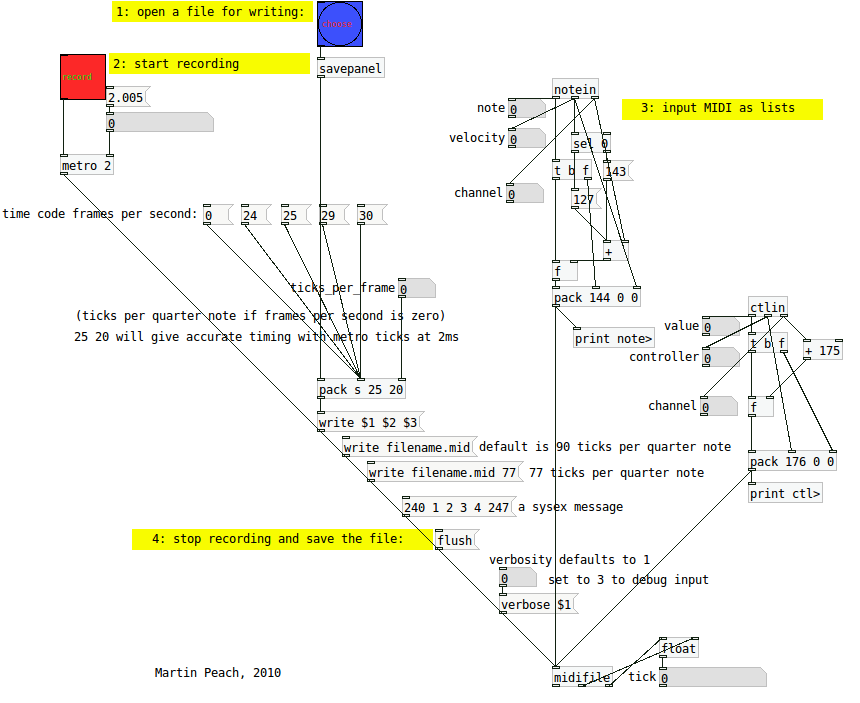
\includegraphics[scale=0.6]{OMPD/PD-midifile_write_-mrpeach.png}
	\end{center}
	\legend{Fonte: autor }
\end{figure}





\subsubsection{Biblioteca [RTC-lib]}


A biblioteca "Real Time Composition" de Karheinz Essl, implementa algumas operações inspiradas em procedimentos seriais, algumas funções inclusive com nomes similares as do Open Music.

\begin{figure}[!h]
	\caption{\label{fig_grafico}Objetos da biblioteca "Real Time Composition" para PD.}
	\begin{center}
	    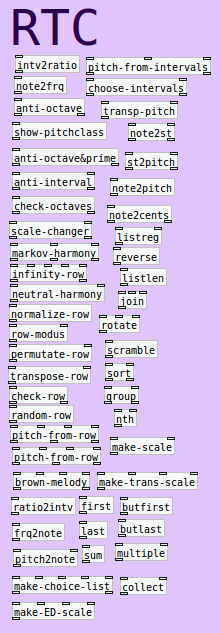
\includegraphics[scale=0.7]{OMPD/PD-RTC.png}
	\end{center}
	\legend{Fonte: autor }
\end{figure}

\subsubsection{Biblioteca de manipulação de listas [list-abs]}

Biblioteca que implementa diversas funções para busca, substituição, operações matemáticas, conversões de tipos, permutações e composições de listas de dados em forma de mensagens PD.

\begin{figure}[!h]
	\caption{\label{fig_grafico}Objetos da biblioteca "list-abs" para PD.}
	\begin{center}
	    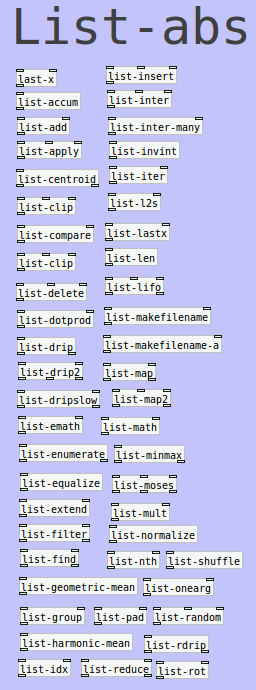
\includegraphics[scale=0.7]{OMPD/PD-list-abs.png}
	\end{center}
	\legend{Fonte: autor }
\end{figure}



\subsubsection{objeto [probalizer]}

Interessante implementação gráfica de histogramas que podem ser alimentados em tempo real, gerando números dentro da mesma probabilidade, encontrado na biblioteca [Unauthorized].

\begin{figure}[!h]
	\caption{\label{fig_grafico}Objeto [probalizer].}
	\begin{center}
	    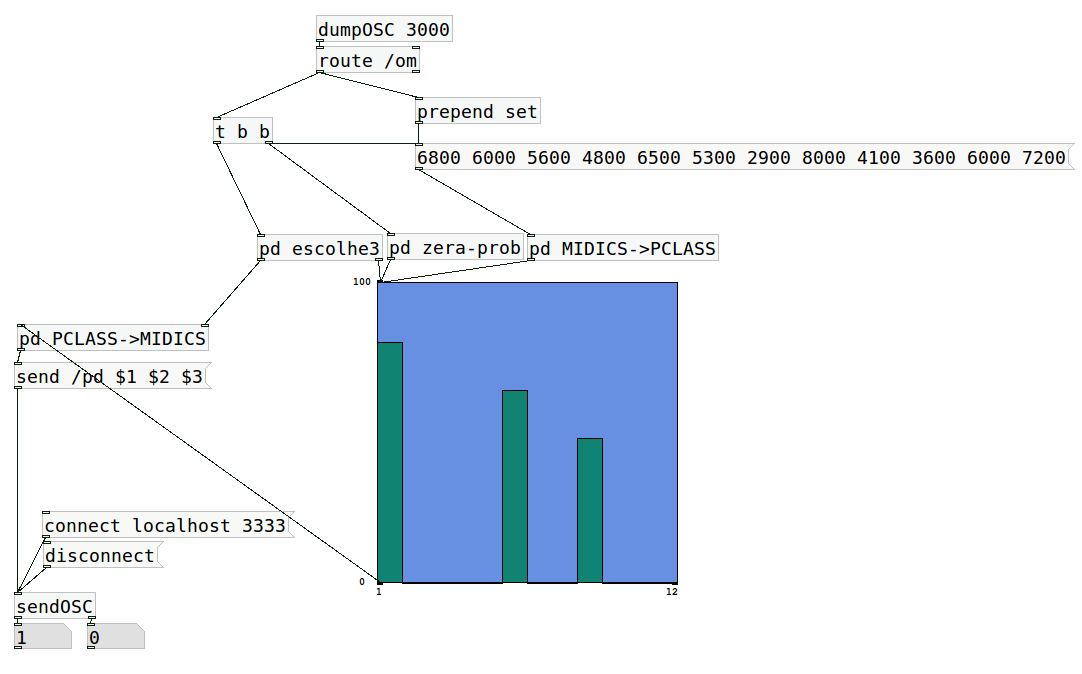
\includegraphics[scale=0.5]{OMPD/Probalizador-PD-OSC-OM.png}
	\end{center}
	\legend{Fonte: autor }
\end{figure}


% ----------------------------------------------------------
\chapter{Arquivos e Scripts para Segmentação de Dados Musicais}
% ----------------------------------------------------------
\label{formatos}

\section{MIDI}

Por muito tempo o formato MIDI ficou estigmatizado por ser associado aos timbres genéricos da indústria de sintetizadores populares dos anos 80 e 90 e pelas primeiras placas de som e softwares sequenciadores de eventos ou partituras dos computadores pessoais. 
Na verdade o formato não carrega parâmetros de timbres em seus metadados. Arquivo MIDI valores básicos de expressão e alturas cromáticas do gestual de uma performance instrumental, permitindo que esta seja posteriormente associada a qualquer timbre.

A mensagem MIDI básica carrega informação sobre:

\begin{enumerate}

\item O canal onde vai atuar permitindo mixar diversos instrumentos em polifonia.

\item O programa que indica o timbre.

\item NoteOn/NoteOff - Nota soando , nota sem soar. o MIDI manda duas informações básicas sobre o envelope da nota. Uma primeira nota com a força inicial e o uma segunda com a mesma nota e força zero, para silenciá-la.

\item "Velocity" ou expressão: força com qual a nota é tocada.

\item Canal de controle para uso de escala de 127 passos que tem uso dependente da implementação da aplicação. Por exemplo, parâmetros de equalização timbre. Na prática o canal de controle é geralmente usado para receber dados de potenciômetros ou sensores analógicos e assinalado a qualquer tipo de parâmetro.

\item Pitch Bend - Parâmetro para atuar diretamente na afinação de uma nota em tempo real, de modo similar ao gesto de bend de instrumentos de cordas. A especificação midi permie que este controle tenha uma granulação de 16.384 pontos e geralmente é usada para um slide que cobre duas oitavas.

\item Mensagens exclusivas de sistema (SysEx) geralmente usadas por aplicações para ações independentes do gesto musical, por exemplo informar ao sistema onde onde buscar arquivos temporários de uma sessão.
\end{enumerate}

É importante ter em mente que os arquivos MIDI, por ser há mais de 35 anos um padrão ainda em uso, gerou um legado relevante de arquivos baseados em repertório clássico para a reconstituição de corpus de peças partituradas. Porém não são descritores capazes de garantir a boa formatação de seus dados como figuras de compasso de uma pauta tradicional, já que os arquivos MIDI não carregam informações sobre as figuras, apenas sobre suas durações, alturas e expressão. Quando importados para programas de notação ou convertidos para formatos destes, os arquivos MIDI irão passar por uma segmentação arbitrária e determinada pelo algoritmo "parser"\footnote{Método computacional para conversão entre formatos ou tipos de dados diferentes.} que vai converter determinada duração em determinada métrica quantizada, normalmente diferente das articulações de quais as músicas foram digitalizadas.


Veremos a seguir outros arquivos mais específicos para este fim e quando necessário será feita a conversão entre os tipos.



\pagebreak

\section{Lilypond}

O objetivo principal aqui é a formatação de uma notação partitural avançada e otimizada para impressão em papel. Permite também a utilização de elementos de notação mais exótica, inclusão de texto, dedilhados, nomenclatura de acordes, sinais de expressão, e customização de elementos a partir de módulos. Facilita a otmização da disposição e dimensão das fontes dos objetos e possui uma linguagem script própria dialeto da sintaxe scheme\footnote{Tutorial oficial de lilypond-scheme: \url{http://lilypond.org/doc/v2.16/Documentation/source/Documentation/extending/introduction-to-scheme} Acesso em 10 de julho de 2014.}.



\begin{figure}[htb]
	\caption{\label{fig_grafico}Gerador de um acorde Dó maior (dó4 e4 g5) na clave de sol em Lilypond}
	\begin{center}
	    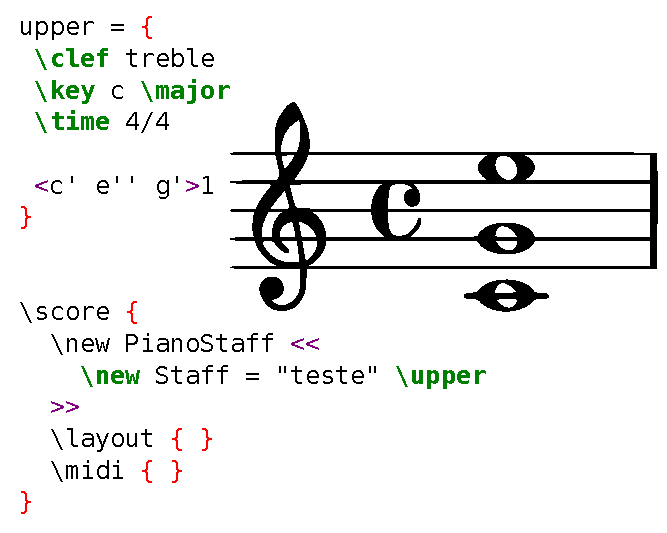
\includegraphics[scale=0.75]{score/lilypond.pdf}
	\end{center}
	%\legend{Fonte: autor}
\end{figure}




\section{MusicXML}

O uso geral do formato MusicXML é similar ao Lilypond - formatação de partituras. No entanto, enquanto Lilypond é um sistema completo fechado em si próprio, o MusicXML é um formato com a intenção de tornar-se um padrão intercambiável entre diferentes aplicações de partitura\footnote{ Lista atualizada de aplicações compatíveis com o formato MusicXML: \url{http://www.musicxml.com/software/} Acesso em 10 de julho de 2014.}.


\begin{figure}[htb]
	\caption{\label{fig_grafico}Gerador de uma nota dó4 na clave de sol em MusicXML}
	\begin{center}
	    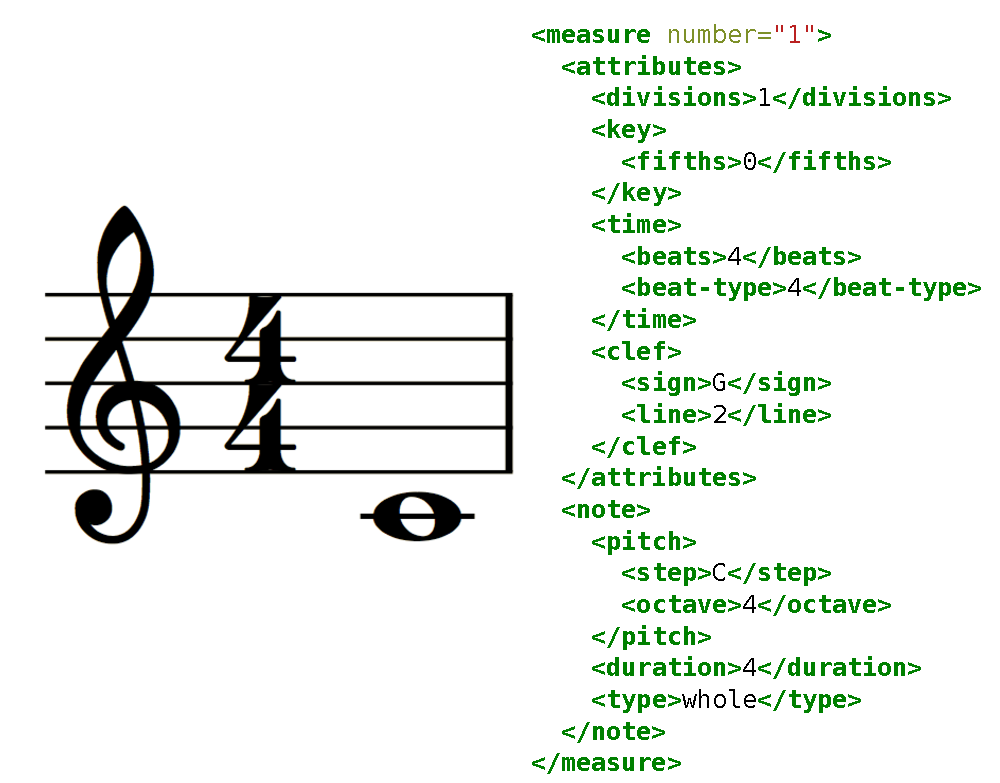
\includegraphics[scale=0.5]{score/musicxml.pdf}
	\end{center}
	%\legend{Fonte: autor}
\end{figure}

\pagebreak
\section{Bibliotecas Python auxiliares}

Pela sua natureza de código aberto alto-nível de orientação a objetos, Python\cite{van1995python} é uma linguagem script que tem sido amplamente adotada e ampliada por bibliotecas para as mais diversas aplicações científicas e artísticas.\cite{downey2009python,Kroger201208}

Aliada ao uso de algumas bibliotecas específicas para arquivos de segmentação partitural, Python mostra-se uma ferramenta prática para formatação dinâmica de partituras prontas para impressão ou para auxiliar a análise de dados quantitativos de corpus de partituras.

Falaremos a seguir de duas dessas bibliotecas utilizadas como ferramenta auxiliar nesta pesquisa:


\subsection{Abjad}

É uma biblioteca voltada para a formatação de clichês em notação partitural pronta para impressão em papel, baseada na manipulação de templates no formato lilypond. A biblioteca apresenta alguns templates baseados em peças de Bártok, Ligeti, Ferneyhough e Mozart.\footnote{\url{http://abjad.mbrsi.org/examples/index.html} Acesso em 10 de julho de 2014.}



\subsection{Music 21}

É uma biblioteca projetada para trabalhar com manipulação e análise de corpus de arquivos partituráveis\footnote{\url{http://web.mit.edu/music21/doc/moduleReference/moduleCorpus.html} Acesso em 10 de julho de 2014.}. Prepara a conversão entre diversos arquivos de dados musicais (midi, humdrum, lilypond, abc)\footnote{\url{http://web.mit.edu/music21/doc/moduleReference/moduleConverter.html} Acesso em 10 de julho de 2014.}, mas nativamente trabalha com uma estrutura de dados baseada em musicxml.

Music21 tem uma abordagem voltada para uma "musicologia assistida por computador" e já tem incorporada em suas classes algumas ferramentas comuns a esta prática como: numeração de grau funcional de acorde\footnote{\url{http://web.mit.edu/music21/doc/moduleReference/moduleRoman.html} Acesso em 10 de julho de 2014.}, numeração de classes de altura usando a classificação de Allen Forte\footnote{\url{http://web.mit.edu/music21/doc/moduleReference/moduleChord.html?\#music21.chord.Chord.forteClassNumber} Acesso em 10 de julho de 2014.} e a implementação dos algoritmos de detecção de tonalidade\footnote{\url{http://web.mit.edu/music21/doc/moduleReference/moduleAnalysisDiscrete.html} Acesso em 10 de julho de 2014.} elaborado por \citeonline{krumhansl1990cognitive} e aperfeiçoado por \citeonline{temperley2001cognition}, descritos nesta pesquisa.\footnote{\autoref{perfiltonal}}


% ---

% ---
% Conclusão (outro exemplo de capítulo s


% ---

% ---
% Conclusão (outro exemplo de capítulo sem numeração e presente no sumário)
% ---em numeração e presente no sumário)
% ---
\chapter*[Conclusão]{Conclusão}
\addcontentsline{toc}{chapter}{Conclusão}
\label{conclusao}
% ---

%\lipsum[31-33]

A busca por regras gerativas\cite{roads1979grammars} que pudessem formalizar algoritmos a partir de análises musicais de dados quantitativos capazes de segmentar e isolar parâmetros nos levou a encontrar uma interessante diferença entre duas abordagens analíticas que nos parecem complementares, apesar de contraditórias em certos aspectos.

Por um lado revisamos uma corrente teórica que enumera estruturas operantes nas expectativas da música tonal, sobre aquele repertório considerado como prática comum nas análises funcionais das cadências, modulações, prolongamentos, tensão e relaxamento. Tais teorias argumentam que esta normatização é derivada de um condicionamento cultural na escuta da música ocidental e procura justificar suas regras de "boa-formação" ou "preferência"\cite{lerdahl1983generative,temperley2001cognition} legitimando as fórmulas a partir de teorias como as teses linguísticas das estruturas de sintaxe derivadas da fala e escrita\cite{chomsky1957syntactic} e pesquisas de campo em cognição musical básica das relações entre intervalos e percepção subjetiva das alturas em seu espaço tonal inferido pelo ouvinte\cite{krumhansl1990cognitive,lerdahl2001tonal}. 

Por outro lado nos chamou atenção que paralelo a fundamentação destas teorias, nas últimas décadas do século XX (e a partir da sedimentação de uma tradição pós-tonal iniciada nas suas primeiras décadas) formalizou-se uma "teoria de grupos das classes de altura"\cite{forte1973structure,rahn1980basic,perle1990pitch,straus2004} baseada numa catalogação de combinações de intervalos formando compostos sonoros singulares e as possíveis estruturações e articulações entre estes. Ali operariam critérios não necessariamente tão amarrados na funcionalidade dos esquemas de tensão e relaxamento das formas "tonalizantes". Mesmo que vertiginosamente, é preciso admitir que cada composição já pode comportar um sistema totalmente idiossincrático. Ao contrário da corrente cognitivista, neste caso uma criatividade autoral do analista assume que as formas estão emergindo ali a príncipio porque foram apontadas, e não necessáriamente porque foram intuídas pelo compositor. Também não buscam justificar expectativas do ouvinte que guiariam a normatização de uma busca composicional da "boa forma" pré-concebida.\cite{babbitt1958cares}

Dadas estas duas perspectivas pretendemos continuar este trabalho com uma organização dos algoritmos sugeridos por estas em bibliotecas das linguagens de programação apontadas na \autoref{computacional}, incluindo aí aprofundar e apontar boas práticas nas linguagens almejando um bom uso destas teorias em processos composicionais. Nos interessa testar os limites práticos destas implementações, deixando um legado tecnicamente viável e acessível, utilizando ferramentas e bibliotecas auxiliares disponíveis em software livre.

Utilizaremos para exemplificar o uso das regras observadas em contextos tonais e pós-tonais alguns aspectos dos algoritmos atuando em um corpus de peças do repertório da suíte Mikrokosmos de Béla Bártok que será revisado no formato musicxml para o estudo computacional, buscando respeitar a grafia das partituras originais. 

Partiremos de pistas já deixadas por autores que aprofundaram o tema \cite{marshall1946analysis,suchoff1971guide, lendvai1971bela,antokoletz1984music,suchoff2004bartok,lester1989analytic}.

Mais do que encontrar alguma nova abordagem analítica sobre estas peças, buscaremos a demonstração de algumas regras gerativas observadas para em seguida serem utilizados de maneira mais livre em procedimentos composicionais que gerem motivos partiturados e sugestões de encadeamento destes.

Composições produzidas durante esta pesquisa estão disponíveis para download\footnote{\url{http://http://vimeo.com/16175509} Acesso em 10 de julho de 2014.}. Também estão disponíveis os códigos que estão sendo trabalhados\footnote{\url{https://github.com/glerm/luteriaOM}, \url{https://github.com/glerm/Derivas_OpenMusic} e \url{https://github.com/glerm/AutomatosGeradores} Acesso em 10 de julho de 2014. }. A próxima etapa será modularizar e comentar os códigos, detalhando os processos de maneira mais didática.

Vale lembrar de que estamos convencidos de que uma abordagem analítica que desconsidere paramêtros determinantes sobre a sonoridade\cite{guigue2012} dos aglomerados de alturas como parte intencional e determinante na composição estará incompleta. Também acreditamos que é limitador ignorar a tipo-morfologia\cite{shaeffer1966traite} e espectro-morfologia\cite{smalley1997spectromorphology} dos timbres atuantes numa situação real de gravação, performance partiturada ou improviso sobre as estruturas geradas. Interessa-nos refletir estes aspectos em alguma continuidade deste trabalho.




% ----------------------------------------------------------
% ELEMENTOS PÓS-TEXTUAIS
% ----------------------------------------------------------
\postextual
% ----------------------------------------------------------

% ----------------------------------------------------------
% Referências bibliográficas
% ----------------------------------------------------------
%\bibliography{abntex2-modelo-references}
\bibliography{mestrado_glerm}
% ----------------------------------------------------------
% Glossário
% ----------------------------------------------------------
%
% Consulte o manual da classe abntex2 para orientações sobre o glossário.
%
%\glossary

% ----------------------------------------------------------
% Apêndices
% ----------------------------------------------------------

% ---
% Inicia os apêndices
% ---
%\begin{apendicesenv}

% Imprime uma página indicando o início dos apêndices
%\partapendices




%%%%

%\chapter{Repositório de Códigos}
%\label{codigo}


%\subsection{Biblioteca de Algoritmos}



%\lstset{frameround=fttt,language=Python,showspaces=false,
%showtabs=true,tab=\rightarrowfill}
%\begin{lstlisting}[frame=trBL]
%def mod12(n):
%	return n % 12
%
%def note_name(number):
%	notes = "C  D E F G A B".split()
%	return notes[mod12(number)]
%	
%for i in intervalos:
%	if (i in maiores):
%		if (i == (4,7)):
%			tipos.append(("maior",0))
%		if (i == (5,9)):
%			tipos.append(("maior",1))
%		if (i == (3,8)):
%			tipos.append(("maior",2))
% 
%	if (i in menores):
%		if (i == (3,7)):
%			tipos.append(("menor",0))
%		if (i == (5,8)):
%			tipos.append(("menor",1))
%		if (i == (4,9)):
%			tipos.append(("menor",2))
%	if (i in aumentados):
%			tipos.append(("aumentado","not"))
%	if (i in diminutos):
%		if (i == (3,6)):
%			tipos.append(("diminuto",0))
%		if (i == (6,9)):
%			tipos.append(("diminuto",1))
%		if (i == (3,9)):
%			tipos.append(("diminuto",2))
% 
%\end{lstlisting}





%\end{apendicesenv}
% ---


% ----------------------------------------------------------
% Anexos
% ----------------------------------------------------------

% ---
% Inicia os anexos
% ---
%\begin{anexosenv}

% Imprime uma página indicando o início dos anexos
%\partanexos



% ---
%\chapter{Regras da Teoria Gerativa da Musica Tonal}
% ---


%\end{anexosenv}

%---------------------------------------------------------------------
% INDICE REMISSIVO
%---------------------------------------------------------------------
\phantompart
\printindex
%---------------------------------------------------------------------

\end{document}
